%!TEX root = tutorial02-slidesonly.tex
%!TEX root = tutorial02-splitshow.tex



%%%%%%%%%%%%%%%%%%%%%%%%%%%%%%%%%%%%%%%%%%%%%%%%%%
%% IMPORTANT:
%% IN ORDER NOTES TO WORK WELL YOU HAVE TO ADD A NOTE TO EACH SLIDE!!!!
%% That is, at least a \emptynote command must be added to each slide.
%%%%%%%%%%%%%%%%%%%%%%%%%%%%%%%%%%%%%%%%%%%%%%%%%%

%\transdissolve

%	\setbeamercolor{postit}{fg=black,bg=yellow}
%	\begin{beamercolorbox}[sep=1em,wd=5cm]{postit}
%	Place me somewhere!
%	\end{beamercolorbox}


\usepackage{etex}
\usepackage[absolute,overlay]{textpos}
\usepackage{pdfsync, xspace}
\usepackage{pstricks,pst-node}
\usepackage{multimedia}
\usepackage[normal,tight,center]{subfigure}
\setlength{\subfigcapskip}{-.5em}
\usefonttheme[onlymath]{serif}

\mode<article> % only for the article version
{
  \usepackage{fullpage}
  \usepackage{hyperref}
}



\mode<presentation>
{
%  \setbeamertemplate{background canvas}[vertical shading][bottom=red!10,top=blue!10]
%  \setbeamertemplate{background canvas}
%  \usetheme{CambridgeUS}
  \usetheme{Boadilla}
}

%  There is a VERY rich set of possible
%  styles of presentations and color themes.  See the
%  beamer documentation for a full list of possibilities.
%\usetheme{Warsaw}  % JuanLesPins  Rochester
%\usetheme{JuanLesPins}

           %  Berkeley  Palo Alto    with sidebar and top
           % Goettingen  Marburg     with sidebar
           %  Copenhagen  Luebeck  Warsaw
%\usecolortheme{lily}
%\usecolortheme{default}
%\usecolortheme{crane}
\usecolortheme{beaver}


\usepackage{times}
\usepackage{multicol}
\setbeamercovered{dynamic}

%\usepackage{pgfarrows}
%  Don't need to load the pgf package, but it has
%  has itself some packages you might want, such as
%  pgfarrows,,pgfnodes,pgfautomata,pgfheaps
%  See the pgf documentation.


% \beamertemplatetransparentcovereddynamic
        % overlays that are upcoming are transparent, in
        % a manner that depends upon how far ahead  they are.


% \beamertemplatetransparentcovereddynamic
        % overlays that are upcoming are transparent, in
        % a manner that depends upon how far ahead  they are.

%\usepackage{beamerthemesplit}
%\usepackage{beamerthemebars}
% beamerthemelined
% beamerthemetree
% beamerthemetreebars
% Note: must be compiled with PDFLatex!!

%\usepackage{graphicx}
% support for Hungarian
%\usepackage[magyar]{babel}
%\usepackage[latin2]{inputenc}

%!TEX root = tutorial01-splitshow.tex


\usepackage[textwidth=\marginparwidth]{todonotes}
\usepackage{pdfsync}
\usepackage{hyperref}
\usepackage{fancybox}

% For citations
\newif\ifnumcites
%\numcitestrue
\numcitesfalse




% The paper has an extended (long) version and a short version
\newif\iflong % Sometimes we want to keep two versions; a short and a long one -- this is useful for that..
%\longfalse
\longtrue

% Turn on/off notes and descriptions of research problems
\newif\ifcomm
%\commfalse % also turns off internal todo comments
%\commtrue

% Turn on/off internal todo comments
\newif\iftodo
\todofalse
%\todotrue


\ifnumcites
  \usepackage[numbers]{natbib}
  \bibliographystyle{plainnat}
\else
  \usepackage{natbib}
  \bibliographystyle{apalike}
\fi
%\bibliographystyle{apalike}
% plain, acm, ieeetr, alpha, acm, abbrv, siam
% plainnat.bst, abbrvnat.bst and unsrtnat.bst
% http://web.reed.edu/cis/help/LaTeX/bibtexstyles.html

\if0
\newcommand{\citep}[1]{\cite{#1}}
\newcommand{\citet}[1]{\cite{#1}}
\newcommand{\citealt}[1]{\cite{#1}}
\newcommand{\iftextcite}[1]{}

\newcommand{\npcite}[1]{\cite{#1}}
\newcommand{\yrcite}[1]{\cite{#1}}
\fi



%\usepackage{amsthm}

\usepackage{amssymb}
%\usepackage[dvips]{graphics}
\usepackage{amsmath,amsthm,amsfonts} % Learn about the AMS package, again very useful!

\usepackage{graphicx}
\usepackage{epstopdf}
\usepackage{stmaryrd}
\usepackage{dsfont}
%\usepackage{small-headings}


\newif\ifshort
\iflong
	\shortfalse
\else
	\shorttrue
\fi


% THEOREMS -------------------------------------------------------
\theoremstyle{plain}
\newtheorem{thm}{Theorem}
\newtheorem{cor}[thm]{Corollary}
\newtheorem{lem}[thm]{Lemma}
\newtheorem{prop}[thm]{Proposition}
\newtheorem{conj}[thm]{Conjecture}
\newtheorem{proofthm}{Proof of Theorem 2}

%\renewtheorem{definition}[thm]{Definition}
\theoremstyle{definition}
\newtheorem{defn}{Definition}
%\theoremstyle{remark}


\newtheoremstyle{example}% ?name? 
{3pt}%	?Space above? 
{3pt}%	?Space below? 
{\itshape}%	?Body font?
{}%	?Indent amount?1 
{}% ?Theorem head font? 
{:}%	?Punctuation after theorem head? 
{.5em}%	?Space after theorem head?2 
{}%
\theoremstyle{example}
\newtheorem{ex}{Example}
%\newtheorem{fact}{Fact}
\newtheorem{rem}{Remark}

\newcounter{assumption}%[section]
\newcommand{\theassumptionletter}{A}
\renewcommand{\theassumption}{\theassumptionletter\arabic{assumption}}

\newenvironment{ass}[1][]{\begin{trivlist}\item[] \refstepcounter{assumption}%
 {\bf Assumption\ \theassumption\ #1} }{%\par\nobreak\noindent\sl\ignorespaces}{%
 \ifvmode\smallskip\fi\end{trivlist}}
\newcommand{\aref}[1]{(\ref{#1})}
\newenvironment{ass*}[1][]{\begin{trivlist}\item[] %
 {\bf Assumption\  #1} }{%\par\nobreak\noindent\sl\ignorespaces}{%
 \ifvmode\smallskip\fi\end{trivlist}}


%\newenvironment{remark}
\newtheorem{remark}{Remark}

%\newenvironment{proof}{{\bf Proof.}}{\hfill\rule{2mm}{2mm}\\}

% Keep whatever you need from here


\newcommand{\norm}[1]{\left\Vert#1\right\Vert}
\newcommand{\smallnorm}[1]{\|#1\|}
\newcommand{\abs}[1]{\left\vert#1\right\vert}
\newcommand{\supnorm}[1]{\norm{#1}_\infty}

\newcommand{\set}[1]{\left\{#1\right\}}
\newcommand{\cset}[2]{\left\{\,#1\,:\,#2\,\right\}}

\renewcommand{\natural}{\mathbb N}                   % Natural numbers
\newcommand{\Real}{\mathbb R}                        % Real numbers
\newcommand{\real}{\mathbb R}                        % again..
\newcommand{\R}{{\mathbb{R}}}                        % again..

\newcommand{\Prob}[1]{{\mathbb P}\left(#1\right)}    % Probabilities; example: \Prob{X>\eps}<1-\delta
\renewcommand{\P}{{\mathbb P}}                         % Probabilities when we want to control the parenthesis
\newcommand{\EE}[1]{{\mathbb E}\left[#1\right]}      % Expectations
\newcommand{\E}{{\mathbb E}}                         % Expectations  when we want to control the parenthesis
\newcommand{\Var}[1]{{\mathrm{Var}}\left[#1\right]}  % Variances
%\newcommand{\one}{\mathbb I}
\newcommand{\one}[1]{{\mathbb I}_{\{#1\}}}           % Characteristic function

\newcommand{\MB}{\mathcal{B}}
\newcommand{\MA}{\mathcal{A}}
\newcommand{\MS}{\mathcal{S}}
\newcommand{\MF}{\mathcal{F}}
\newcommand{\MC}{\mathcal{C}}
\newcommand{\MRR}{\mathcal{R}}
\newcommand{\MD}{\mathcal{D}}
\newcommand{\MP}{\mathcal{P}}
\newcommand{\MU}{\mathcal{U}}
\newcommand{\MO}{\mathcal{O}}
\newcommand{\MX}{\mathcal{X}}
\newcommand{\GG}{\mathcal{G}}
\newcommand{\hZ}{\hat{Z}}
\newcommand{\hF}{\hat{F}}
\newcommand{\hL}{\hat{L}}
\newcommand{\tL}{\tilde{L}}

\newcommand{\MI}{{\bf I}} %\mathbb{I}}


\newcommand{\eps}{\varepsilon}                       % Nice epsilon
\newcommand{\ep}{\varepsilon}                        % Shorthand for nice epsilon
\newcommand{\de}{\delta}                             % Shorthand for delta
\newcommand{\To}{\longrightarrow}
\newcommand{\ra}{\rightarrow}

\newcommand{\argmin}{\mathop{\rm argmin}}
\newcommand{\argmax}{\mathop{\rm argmax}}
\newcommand{\diag}{\mathop{\rm diag}}
\newcommand{\inlinemin}{\wedge}
\newcommand{\inlinemax}{\vee}

\newcommand{\ip}[2]{\langle #1,#2\rangle}
\newcommand{\bigip}[2]{\Big\langle #1,#2\Big\rangle}
\newcommand{\eqdef}{\stackrel{\mbox{\rm\tiny def}}{=}}
\newcommand{\aP}{{\cal P}}

% Shorthands I use for math environments
\newcommand{\beq}{\begin{equation}}
\newcommand{\eeq}{\end{equation}}
\newcommand{\beqa}{\begin{eqnarray}}
\newcommand{\eeqa}{\end{eqnarray}}
\newcommand{\beqan}{\begin{eqnarray*}}
\newcommand{\eeqan}{\end{eqnarray*}}
\newcommand{\ben}{\begin{eqnarray*}}
\newcommand{\een}{\end{eqnarray*}}

\newcommand{\RA}{$\Rightarrow$}

\newcommand{\TODO}[2][]{\todo[#1]{#2}}

\iflong
\else
	\renewcommand{\note}[2][]{}
	\renewcommand{\bibnote}[2][]{}
	\renewcommand{\problem}[2][]{}
\fi

\ifcomm
   \newcommand\comm[1]{\textcolor{blue}{ #1}}
\else
   \newcommand\comm[1]{}
%   \renewcommand{\todo}[1]{}
   \renewcommand{\todo}[2][]{}
\fi

\iftodo
\else
  \renewcommand{\TODO}[2][]{}
\fi

\newcommand{\remove}[1]{\textcolor{blue}{\sout{#1}}}
\newcommand{\tO}{\tilde{O}}

% Boldfaced lowercase greek letters as described at
% http://www.rpi.edu/dept/acs/rpinfo/common/Computing/Consulting/Software/LaTeX/Hints/Greek_Chars.html
\def\bmath#1{\mbox{\boldmath$#1$}}
% http://www.ctan.org/tex-archive/info/symbols/comprehensive/symbols-a4.pdf page 68
\newcommand\independent{\protect\mathpalette{\protect\independenT}{\perp}}
\def\independenT#1#2{\mathrel{\rlap{$#1#2$}\mkern2mu{#1#2}}}


\newcommand{\Set}{S}
\newcommand{\States}{\mathcal{X}}
\newcommand{\Actions}{\mathcal{A}}
\newcommand{\TranKernel}{\mathcal{P}}
\newcommand{\JTranKernel}{\mathcal{P}_{0}}
\newcommand{\PKernel}{\mathcal{P}}
\newcommand{\RKernel}{\mathcal{Q}}
\newcommand{\st}{x}
\newcommand{\St}{X}
\renewcommand{\action}{a}
\newcommand{\nextaction}{a'}
\newcommand{\Action}{A}
\newcommand{\Nextaction}{A'}
\newcommand{\reward}{r}
\newcommand{\Reward}{R}
\newcommand{\Ret}{\mathcal{R}}
\newcommand{\MDP}{\mathcal{M}}
\newcommand{\nextstate}{y}
\newcommand{\Nextstate}{Y}
\newcommand{\rewardfun}{r}
\newcommand{\TransPOp}{P}
\newcommand{\id}{I}

\renewcommand{\atop}{^{\top}}
\newcommand{\SA}{\States\times\Actions}


\newcommand{\astate}{z}
\newcommand{\AStates}{Z}%\State_A}
\newcommand{\APKernel}{\PKernel_A}
\newcommand{\rewardrange}{{\mathcal R}}
\iflong
\newcommand{\myfootnote}[1]{\footnote{#1}}
\else
\newcommand{\myfootnote}[1]{}
\fi
\renewcommand{\epsilon}{\varepsilon}

\newcommand{\tder}{\nabla_\theta}
\newcommand{\tders}{\nabla_\theta}
\newcommand{\pder}{\frac{\partial}{\partial \theta}}
\newcommand{\pders}{\tfrac{\partial}{\partial \theta}}


\newcommand{\pai}{{(i)}}
\newcommand{\integer}{\mathbb{Z}}
\newcommand{\cD}{{\cal D}}
\newcommand{\cZ}{{\cal Z}}
\newcommand{\cX}{{\cal X}}
\newcommand{\cW}{{\cal W}}

\newcommand{\cG}{{\cal G}}
\newcommand{\cF}{{\cal F}}
\newcommand{\cH}{{\cal H}}
\renewcommand{\phi}{\varphi}
\newcommand{\ewithin}{\eps_{\text{W}}}
\newcommand{\ebetween}{\eps_{\text{B}}}
\newcommand{\emean}{\eps_{\text{M}}}
\DeclareMathOperator{\trace}{trace}
\newcommand{\e}{\mathbf{1}}
\renewcommand{\eps}{\varepsilon}
\newcommand{\cM}{{\cal M}}
\newcommand{\cS}{{\cal S}}
\newcommand{\tM}{\tilde{M}}
\newcommand{\MRP}{{\cal M}}
\newcommand{\kfun}{\mathbb{K}}
\newcommand{\cK}{{\cal K}}

\newcommand{\aparam}{\omega}
\newcommand{\dimaction}{d_{\Actions}}
\newcommand{\dimaparam}{d_{\aparam}}
\newcommand{\traj}{\xi}
\newcommand{\Trajset}{\Xi}
\newcommand{\Traj}{X}
\newcommand{\perf}{\rho}
\newcommand{\dstat}{\mu} % stationary distribution underlying a Markov chain
\newcommand{\Regret}{{\bf R}}
\renewcommand{\AA}{{\cal A}}
%\newcommand{\SA}{\States\times\Actions}
\newcommand{\Sample}{{\cal D}}
\newcommand{\hA}{\hat{A}}
\newcommand{\hb}{\hat{b}}
\newcommand{\ZZ}{{\cal Z}}
\newcommand{\ttop}{^\top}
\newcommand{\FF}{{\cal F}}
\newcommand{\PiStat}{\Pi_{\rm stat}}
\newcommand{\td}{\delta}
\newcommand{\hV}{\hat{V}}
\newcommand{\mynote}[1]{}
\newcommand{\elg}{z}
\newcommand{\furtherreading}{}
\newcommand{\rfun}{\reward}
\newcommand{\pscorefun}[1]{\frac{\partial \ln \pi_\aparam(#1)}{\partial \aparam}}
\newcommand{\pscorefunp}[1]{\frac{\partial}{\partial\aparam}\,\log \pi_\aparam(#1)}
\newcommand{\scorefun}{\psi}
\newcommand{\hQ}{\hat{Q}}
\renewcommand{\th}{^{\rm th}}
\newcommand{\bee}{\begin{enumerate}}
\newcommand{\eee}{\end{enumerate}}

\usepackage{algorithm}
\usepackage{algpseudocode}
\algnewcommand\algorithmicto{\textbf{to}}
\algnewcommand\algorithmicdownto{\textbf{downto}}

%!TEX root = tutorial01-splitshow.tex

\usepackage{wasysym} % for \smiley \frownie
%
% \usepackage{wrapfig}
% \begin{wrapfigure}{POS}{WIDTH}{LINES TO RESERVE}
% ..
% \end{wrapfigure}
% The last argument is optional

% Figures need exact positioning in columns
% Use the following command to place them
\newcommand{\figincol}[1]{
\pgfputat{\pgfxy(0,0)}{\pgfbox[left,top]{#1}}
}

% ALSO:
% \pgfputat {\pgfxy(XX,YY)}{\pgfbox[left,base]{#1}}
% 
% LL = (0cm,-7cm) 
% UR = (11cm,1cm)
%
% pgfdeclareimage
% pgfuseimage

\newcommand{\Ra}{\Rightarrow}
%% BEAMER SPECIFIC COMMANDS

\newcommand{\bi}{\begin{itemize}}
\newcommand{\ei}{\end{itemize}}
\newcommand{\bc}{\begin{center}}
\newcommand{\ec}{\end{center}}


\setbeamercolor{math text}{fg=blue!50!normal text.fg}
\newcommand{\animframe}[2]{\begin{frame}[<+->]{#1}#2\end{frame}}
\newcommand{\animframesq}[2]{\begin{frame}[<+->][shrink,squeeze]{#1}#2\end{frame}}
\newcommand{\animframejsq}[2]{\begin{frame}[<+->][squeeze]{#1}#2\end{frame}}

\newcommand{\animframen}[2]{\begin{frame}[<+->]{#1}#2\emptynote\end{frame}}
\newcommand{\animframesqn}[2]{\begin{frame}[<+->][shrink,squeeze]{#1}#2\emptynote\end{frame}}
\newcommand{\animframejsqn}[2]{\begin{frame}[<+->][squeeze]{#1}#2\emptynote\end{frame}}

\newcommand{\myframe}[2]{\begin{frame}{#1}#2\end{frame}}
\newcommand{\myframesq}[2]{\begin{frame}[shrink,squeeze]{#1}#2\end{frame}}
\newcommand{\myframejsq}[2]{\begin{frame}[squeeze]{#1}#2\end{frame}}

\newcommand{\myframen}[2]{\begin{frame}{#1}#2\emptynote\end{frame}}
\newcommand{\myframesqn}[2]{\begin{frame}[shrink,squeeze]{#1}#2\emptynote\end{frame}}
\newcommand{\myframejsqn}[2]{\begin{frame}[squeeze]{#1}#2\emptynote\end{frame}}


%\setbeamertemplate{footline}[frame number]
\newtheorem{Solution}[theorem]{Solution}
\newtheorem{Comm}[theorem]{Comment}
\newtheorem{Note}[theorem]{Note}

\newcommand{\bcol}[1][t]{\begin{columns}[#1]} % optional argument: alignment (t,b,c)
\newcommand{\ecol}{\end{columns}}
\newcommand{\col}[1][0.5\textwidth]{\column{#1}} % argument: width of the column
%\parindent = 10pt
\newcommand{\scaletext}[3]{ % scale-factor original-width TEXT
\scalebox{#1}{\begin{minipage}[h]{#2\textwidth} #3 \end{minipage}
}}

% note: beamer slides are 128mm by 96 mm
\newcommand{\putatUL}[4]{ % width xpos ypos WHAT; upper left corner is put at the said pos
\begin{textblock*}{#1}[0,0](#2,#3)
#4
 \end{textblock*}
}
\newcommand{\putatBR}[4]{ % width xpos ypos WHAT; bottom right corner is put at the said pos
\begin{textblock*}{#1}[1,1](#2,#3)
#4
 \end{textblock*}
}
\newcommand{\putatBL}[4]{ % width xpos ypos WHAT; bottom left corner is put at the said pos
\begin{textblock*}{#1}[0,1](#2,#3)
#4
 \end{textblock*}
}
\newcommand{\putatUR}[4]{ % width xpos ypos WHAT; bottom right corner is put at the said pos
\begin{textblock*}{#1}[1,0](#2,#3)
#4
 \end{textblock*}
 }
 \newcommand{\putatMID}[4]{ % width xpos ypos WHAT; bottom right corner is put at the said pos
\begin{textblock*}{#1}[0.5,0.5](#2,#3)
#4
 \end{textblock*}
 }

\newcommand{\putat}[3]{\begin{picture}(0,0)(0,0)\put(#1,#2){#3}\end{picture}} % xrelpos yrelpos WHAT

\makeatletter
\newcommand{\insertprevframe}[1]{
	\def\beamer@origlmargin{\Gm@lmargin}
%    \vbox{\hfill\insertslideintonotes{0.125}\hskip-\Gm@rmargin\hskip0pt%
%      \vskip-0.125\paperheight\nointerlineskip}%
	\insertslideintonotes{#1}
}

%\newcommand{\insertslideintonotes}[1]{{%
%  \begin{pgfpicture}{0cm}{0cm}{#1\paperwidth}{#1\paperheight}
%    \begin{pgflowlevelscope}{\pgftransformscale{#1}}%
%      \color[gray]{0.8}
%      \pgfpathrectangle{\pgfpointorigin}{\pgfpoint{\paperwidth}{\paperheight}}
%      \pgfusepath{fill}
%      \color{black}
%      {\pgftransformshift{\pgfpoint{\beamer@origlmargin}{\footheight}}\pgftext[left,bottom]{\copy\beamer@frameboxcopy}}
%    \end{pgflowlevelscope}
%  \end{pgfpicture}%
%  }}
\makeatother
% For adding items to the notes pages (we do not want animation there)
\newcommand{\bin}{\bi[<1->]}


\title[RL Algorithms]{
Reinforcement Learning Algorithms in Markov Decision Processes\\
AAAI-10 Tutorial\\
\mbox{}\\
Part II: Learning to predict values
}
\author[Szepesv\'ari \& Sutton]{Csaba Szepesv\'ari \and Richard S. Sutton}
\institute[UofA]{
University of Alberta\\
E-mails: {\bf \{szepesva,rsutton\}@.ualberta.ca}\\
}
\date[July 11, 2010]{Atlanta, July 11, 2010}

\begin{document}

\frame{
	\titlepage
	\putatBL{10mm}{10mm}{66mm}{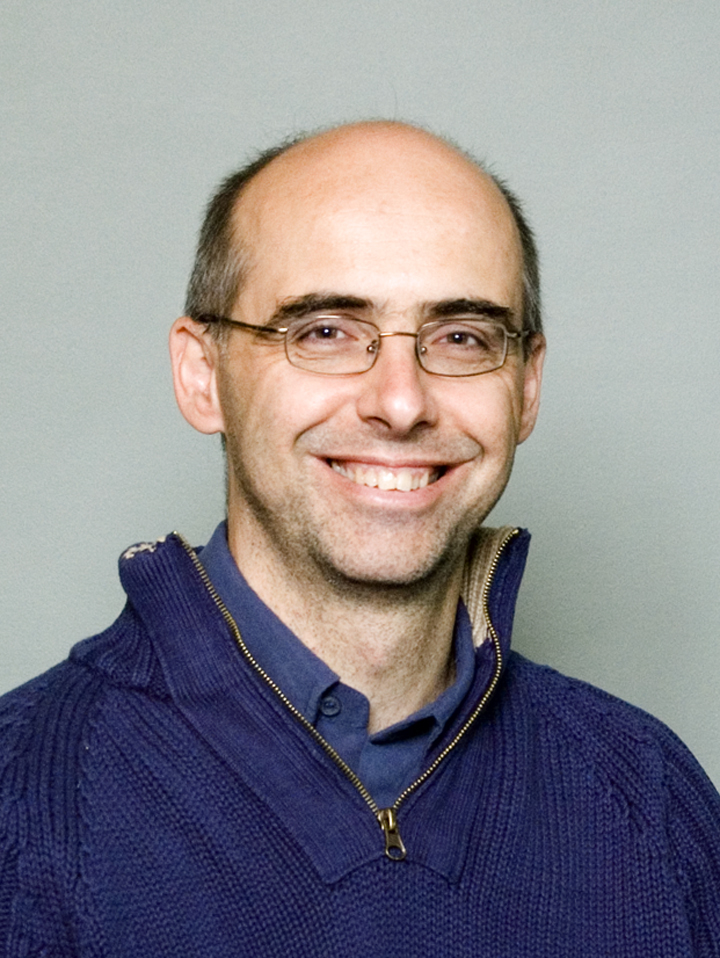
\includegraphics[width=10mm]{Figures/Szepesvari.jpg}}
	\putatBR{10mm}{118mm}{66mm}{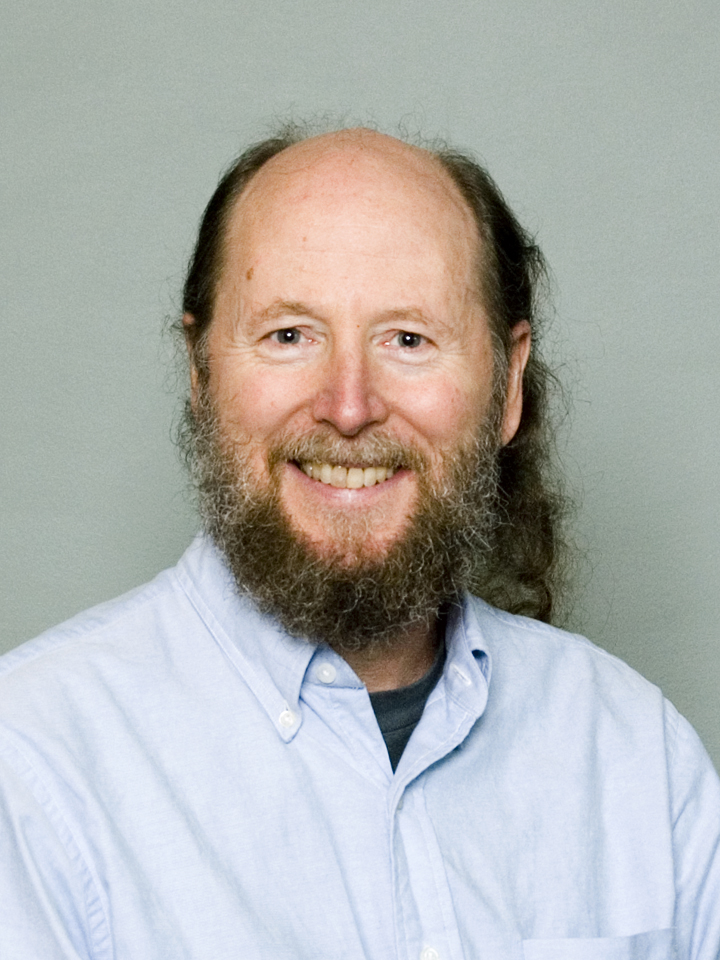
\includegraphics[width=10mm]{Figures/Sutton}}
	% 128 x 96 mm
	\putatMID{20mm}{64mm}{85.5mm}{
	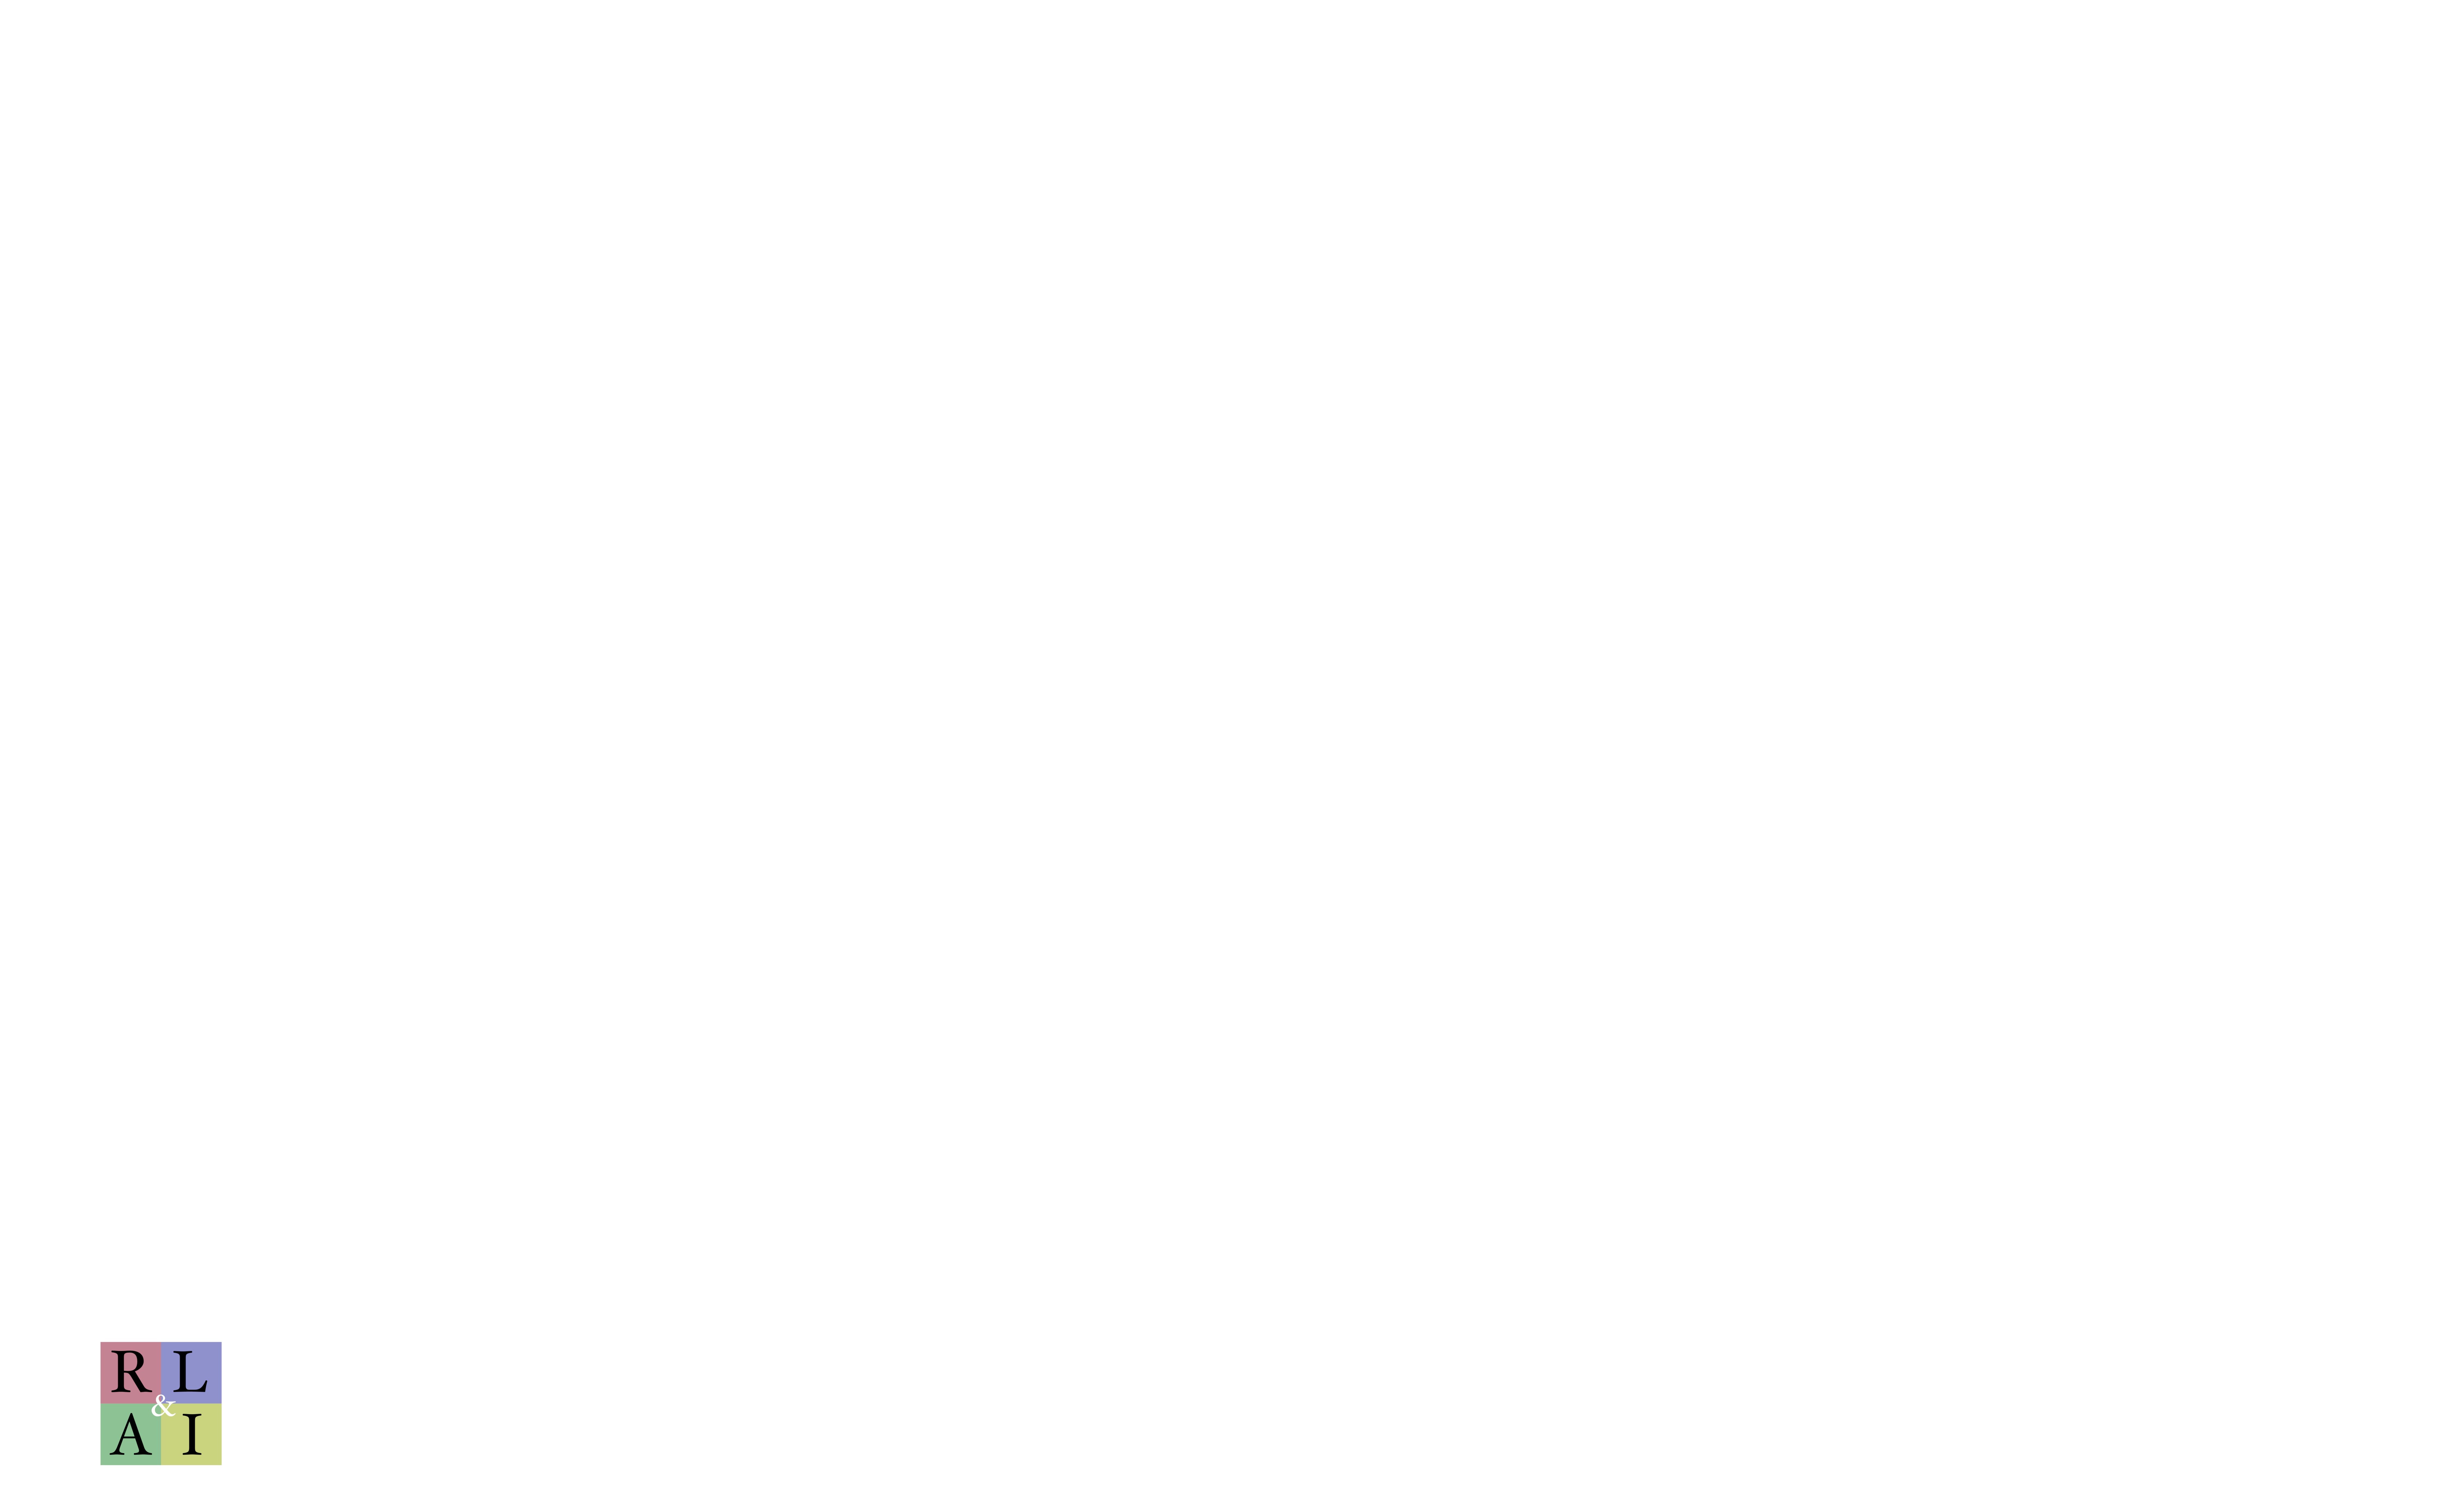
\includegraphics[width=10mm]{Figures/rlai}
	
\includegraphics[width=10mm]{Figures/UofA-lowRes}
	}
	\emptynote
}

%\maketitle
\section<presentation>*{Outline}

\begin{frame}
  \frametitle{Outline}
  %\scriptsize
  \tableofcontents[part=1] %,pausesections]
    \emptynote

\end{frame}

\AtBeginSubsection[]
{
  \begin{frame}<beamer>
    \frametitle{Outline}
    \tableofcontents[current,currentsubsection]
    \emptynote
  \end{frame}
}

\part<presentation>{Main Talk}

\section{Introduction}
\animframen{The problem}
{
\begin{alertblock}{}
\bigskip
\begin{center}
 How to learn the value function of a policy \\
 over a large state space?
 \end{center}
\bigskip
\end{alertblock}

\bcol
\col
Why \alert{learn}?
\bi
\item Avoid the ``curses of modeling''
\bi
\item Complex models are hard to deal with
\item Avoids modelling errors
\item Adaptation to changes
\ei
\ei

\col
Why learn \alert{value functions}?
\bi
\item Applications:
\bi
\item Failure probabilities in a large power grid %\citep{FraMaPre08} 
\item Taxi-out times of flights on airports% \citep{BaGaSheLe08},
\item Generally: Estimating a long term expected value associated with a Markov process
\ei
\item Building block 
\ei
\ecol
\note{
\bin
\item Other applications:
\bin
	\item Predict the yield of a chemical reactor
	\item Predict if the robot is going to fall over
	\item Predict who is going to win in a game
	\item Predict if the robot is going to go through the doorway
\ei
\ei
}
}

\section{Simple learning techniques}

\subsection{Learning the mean}
\animframejsqn{Learning the mean of a distribution}
{
\vspace*{-0.1in}
\bi
\item Assume $\Reward_1,\Reward_2,\ldots$ are i.i.d., $\exists V = \EE{ \Reward_t }$.
\item Estimating the expected value by the sample mean:
\[
V_{t} = \frac1t \sum_{s=0}^{t-1} \Reward_{s+1}.
\]
\item Recursive update:
\[
V_{t} = V_{t-1} + \frac1t \, (\underbrace{\Reward_{t}}_{\mathrm{\alert{``target''}}} - V_{t-1}).
\]
\item More general update:
\[
V_{t} = V_{t-1} + \alpha_t \, (\Reward_{t} - V_{t-1}),
\]
\item ``Robbins-Monro'' conditions:
\[
\sum_{t=0}^\infty \alpha_t = \infty, \qquad \sum_{t=0}^\infty \alpha_t^2 <\infty
\]
\ei
\note{
\tiny
\bin
	\item The mean converges to the expected value assuming that the mean exists.
	\item This is almost sure convergence
	\item The rate of convergence is $t^{-1/2} \sqrt{\Var{R_1}}$, assuming that $\Var{R_1}$ exists
	\item If $R_t$ is bounded (more generally, has sub-Gaussian tails) then we have high-probabiltiy deviation inequalities
	\item The derivation of the recursive update is:
	\beqan
	V_t 
	 &=& \frac1t \left\{ (t-1) V_{t-1} + \Reward_{t} \right\} \\
 	&=& V_{t-1} + \frac1t \, (\Reward_{t} - V_{t-1}).
	\eeqan
	\item The RM conditions:
	\bin \tiny
		\item If $\sum_{t=0}^\infty \alpha_t<\infty$ then not all data is used
		\item The other condition controls the variance
	\ei
	\item The learning rate allows a finer control of the convergence -- important for more complicated cases (not here)
	\item If $\alpha_t \equiv {\rm const}$ small, then we have convergence in distribution to a random variables whose variance is proportional to $\alpha_t = \alpha_1$.
\ei
}
}

\subsection{Learning values with Monte-Carlo}
\animframen{Application to learning a value: \small the Monte-Carlo method}
{
%\begin{block}{Setup}

%\includegraphics[width=3.5in]{mrp3}
\putat{210}{-66}{\includegraphics[width=1.9in]{Figures/mrp3}}
\mbox{}
\bigskip
{\bf Setup:}
\bi
\item Finite, episodic MDP
\item Policy $\pi$, which is proper from $\st_0$
\item Goal: Estimate $V^\pi(\st_0)$!
\item Trajectories:
\beqan
\St^{(0)}_0, \Reward_1^{(0)}, \St^{(0)}_1, \Reward_2^{(0)}, \ldots, \St^{(0)}_{T_0}, \\
\St^{(1)}_0, \Reward_1^{(1)}, \St^{(1)}_1, \Reward_2^{(1)}, \ldots, \St^{(0)}_{T_1}, \\
\vdots 
\eeqan
where $\St^{(i)}_0 = \st_0$
\ei
%\end{block}
\note{
\bin
\item Of course, the trajectories could originate from some other state, too
\item Practical examples: 
\bin
\item Soap bubble, what is the height at a point?
\item What is the temperature in an oven 
\item (PDEs!)
\item Notice: The state space does not have to be finite, since you are interested only the value at one point. At least if you can control where the trajectories originate from. 
\item The point is to overcome the ``curse of modeling''
\ei
\ei
}
}
\begin{frame}
\frametitle{First-visit Monte-Carlo}
	\begin{algorithmic}[1]
	\Statex \mbox{} \hspace*{-2em} {\bf function} \Call{FirstVisitMC}{${\cal T}, V, n$} 
	\Statex \mbox{} \hspace*{-2em} ${\cal T}= (\St_0,\Reward_1, \ldots, \Reward_T, \St_T)$ is a trajectory
	with $\St_0 = \st$ and $\St_T$ being an absorbing state, $n$ is the number of times $V$ was updated
	\State $\mathrm{ sum} \gets 0$
	\For{$t=0$ \algorithmicto   $\; T-1$}
		\State $\mathrm{sum} \gets \mathrm{sum} + \gamma^t \Reward_{t+1}$
	\EndFor
	\State $V \gets V + \frac1n (\mathrm{sum} - V)$
	\State \Return $V$
	\end{algorithmic}

\note{
\bin
\item The variance of the returns can be high \\
	(proportional to the length of the trajectory)
\item $\St_0 = \st$ will not necessarily hold for the initial state, \\
 but then the algorithm can be trivially modified -- as long as the state space is finite
\item Real issue: How to apply this to non-episodic problems? (Bias)
\item This is the \alert{first-visit version}; the \alert{every-visit version} show next updates more often
\item The algorithm throws away too much data, the every-visit seems more data savvy
\ei
}
\end{frame}

\begin{frame}
\frametitle{Every-visit Monte-Carlo -- learning a value function}
        \begin{algorithmic}[1]
        \Statex \mbox{} \hspace*{-2em} {\bf function} \Call{EveryVisitMC}{$\St_0,\Reward_1,\St_1,\Reward_2,\ldots,\St_{T-1},\Reward_T,V$} 
	\Statex \mbox{} \hspace*{-2em} \textbf{Input:} $\St_t$ is the state at time $t$, $\Reward_{t+1}$ is the reward associated with the $t\th$ transition, $T$ is the length of the episode, $V$  is the array storing the current value function estimate
	\State $\mathrm{sum} \gets 0$
	\For{$t\gets T-1$  \algorithmicdownto\ $0$}
		\State $\mathrm{sum} \gets \Reward_{t+1} + \gamma\,\cdot\, \mathrm{sum} $
		\State $\mathrm{target}[\St_t] \gets \mathrm{sum}$
		\State $V[\St_t] \gets V[\St_t] + \alpha\,\cdot\, ( \mathrm{target}[\St_t] - V[\St_t] )$
	\EndFor
	\if0
	\For{$t\gets 1, \ldots, T-1$}
		\State $\Ret \gets 0$
		\For{$s\gets t, \ldots, T-1$}
			\State $\Ret \gets \Ret + \gamma^{s-t} \Reward_{s+1}$
		\EndFor
		\State $V[\St_t] \gets V[\St_t] + \alpha ( \Ret - V[\St_t] )$
	\EndFor
	\fi
	\State 	\Return $V$
	\end{algorithmic}
\note{
\bin
\item This routine must be called at the end of each episode with the state-reward sequence collected during the episode. 
\item The algorithm has linear time- and space-complexity in the length of the episodes.
\item Cannot be used (anymore)  in infinite state spaces; all the values are learned simultaneously
\item These Monte-Carlo methods are called \alert{multi-step} methods as they use multi-step value estimates to update the value estimates
\item \alert{Question}: How to generalize this to learn action values of the state, provided that there are finitely many actions?
\ei
}
\end{frame}


\subsection{Learning values with temporal differences}
\animframen{Learning from snippets of data}
{
\begin{alertblock}{Goals}
\bigskip
\bi
\item Learn from elementary transitions of the form $(\St_t,\Reward_{t+1},\St_{t+1})$
\item Learn a full value function
\item Increase convergence rate (if possible)
\ei
\bigskip
\end{alertblock}

\bigskip
\bigskip
\bigskip
\uncover<+->{
\begin{center}
\Large $\Longrightarrow$ Temporal Difference (TD) Learning
\end{center}
}
\note{ The goal really is to overcome the limitations of Monte-Carlo..}
}
\animframen{Learning from guesses: TD learning}
{
\bi
\item Idealistic Monte-Carlo update:
\[
V(\St_t) \gets V(\St_t) + \frac1t ( \Ret_t - V(\St_t) ),
\]
where $\Ret_t$ is the return from state $\St_t$.
\item However, $\Ret_t$ is not available!
\item \alert{Idea}: Replace it with something computable:
\beqan
\Ret_t 
 &=& \Reward_{t+1} + \gamma \Reward_{t+2} + \gamma^2 \Reward_{t+3} + \ldots \\
 &=& \Reward_{t+1} + \gamma \left\{ \Reward_{t+2} + \gamma \Reward_{t+3} + \ldots \right\} \\
 &\approx& \Reward_{t+1} + \gamma V(\St_{t+1}).
\eeqan
\item Update:
\[
V(\St_t) \gets V(\St_t) + \frac1t 
	\overbrace{\left\{ \Reward_{t+1} + \gamma V(\St_{t+1}) - V(\St_t) \right\}}^{\alert{\delta_{t+1}(V)}}.
\]
\ei
\note{
\bin
\item In general, we can write anything in place of $\Ret_t$ that has the same conditional mean
given state $\St_t$.
\item If $V$ was already the true value function then the update would be correct
\item But it is not, so the update is \alert{biased}
\item However, the \alert{variance} is reduced
\item One can show that the bias disappears in the limit
\item One can also introduce learning rates
\item Here, $\delta_{t+1}(V) = \Reward_{t+1} + \gamma V(\St_{t+1}) - V(\St_t)$ is called a temporal difference.
\item Note that $\EE{ \delta_{t+1}(V) |\St_t = \st} = 0$, $\st\in \States$ is equivalent to the Bellman equation.
\item Also, the update can be written in the form 
\[
V(\st) = V(\st) + \alpha_t \delta_{t+1}(V)\, \one{\St_t = \st}.
\]
\ei
}
}

\begin{frame}
\frametitle{The TD(0) algorithm}

	\begin{algorithmic}[1]
	\Statex \mbox{} \hspace*{-2em} {\bf function} \Call{TD0}{$\St,\Reward,\Nextstate,V$} 
	\Statex \mbox{} \hspace*{-2em} \textbf{Input:} $\St$ is the last state, $\Nextstate$ is the next state, $\Reward$ is the immediate reward associated with this transition, $V$  is the array storing the current value  estimates
	\State $\delta  \gets \Reward+\gamma \,\cdot\, V[\Nextstate] - V[\St]$
	\State $V[\St] \gets V[\St] + \alpha \,\cdot\,\delta$ \label{line:td0update}
	\State \Return $V$
	\end{algorithmic}
\note{
\bin
\item We achieved the goals:
\bin
\item Learns from snippets of data
\item Does not have to wait until the end of the episode
\ei
\item \alert{Question}: How to generalize this to learn action values of the state, provided that there are finitely many actions? What do we have to be careful about? (All state-action pairs visited i.o.)
\item Theory: As long as all states are visited i.o. and the step-sizes satisfy the RM conditions, the values converge to their true values w.p.1.
\bin
\item Version one: Local counter-based step-sizes; no further conditions
\item Version two: Global step-sizes. In this case all states should be visited with positive limiting frequency
\ei
\ei
}
\end{frame}

\setbeamercovered{invisible}

\subsection{Monte-Carlo or TD?}
\myframen{Which one to love? Part I}
{
\begin{center}
\includegraphics[width=3in]{Figures/mrp3}
\end{center}

\bcol
\col
\uncover<2->{
TD(0)  at state $2$:
\bi
\item By the  $k^{\rm th}$ visit to state $2$, state $3$ has already been visited $\approx 10\, k$ times!
\item $\Var{\hV_t(3)} \approx 1/(10\,k)$!
\ei
}
\col
\uncover<3->{
MC at state $2$:
\bi
\item $\Var{\Ret_t|\St_t=2} = 0.25$, does not decrease with $k$!
\ei
}
\ecol

\putatMID{0.5\textwidth}{64mm}{48mm}{
	\uncover<4-|handout:0>{
	\begin{alertblock}{Conclusion}
	\bigskip
	\bc
	Bootstrapping helps!
	\ec
	\bigskip
	\end{alertblock}
	}
}

\note{
	The point is that sometimes learning from guesses is a good thing: You use data more efficiently.
}

}


\myframen{Which one to love? Part II}
{
\begin{center}
\includegraphics[width=3.5in]{Figures/mrp3}
\end{center}

\bi
\item Replace the stochastic reward by a deterministic one of value $1$
\item TD has to wait until the value of $3$ converges
\item MC updates towards the correct value in every step (no variance!)
\ei

\putatMID{0.5\textwidth}{64mm}{48mm}{
	\uncover<3-|handout:0>{
	\begin{alertblock}{Conclusion}
	\bigskip
	\bc
	Bootstrapping does \alert{not} help.. \frownie
	\ec
	\bigskip
	\end{alertblock}
	}
}

\note{
% TODO: replace the figure
\bin
\item
In fact, one can  imagine a longer chain of states, where state $i+1$ follows state $i$, for $i\in \{1,\ldots,N\}$ and the only time a nonzero reward is incurred is when transitioning from state $N-1$ to state $N$. In this example, the rate of convergence of the Monte-Carlo method is not impacted by the value of $N$, while TD(0) would get slower with  $N$ increasing.
\item
The point is that sometimes learning from guesses is harmful as the data may be more precise than the guess. The criterion seems to be that the return should have a low variance on its own. Then learning from guesses will only slow you down since initially the guesses will depend on their initial values and thus can be biased.
\item \alert{Question}: What is a problem class when the variance of return does {\em not} grow unbounded with the length of the trajectory? (Answer: Episodic, with payoff at the end. In the opposite case, i.e., in the case of dense rewards, the variance typically grows with the length.)
\ei
}
}

\setbeamercovered{dynamic}

\subsection{Resolution}
\animframen{The happy compromise: TD($\lambda$)}
{
\bi
\item Choose $0\le \lambda \le 1$
\item Consider the \alert{$k$-step return estimate}:
\[
\Ret_{t:k} = \sum_{s=t}^{t+k} \gamma^{s-t} \Reward_{s+1} \,\, +\,\, \gamma^{k+1} \,\hV_t(\St_{t+k+1}),
\]
\item Consider updating the values toward the so-called \alert{ $\lambda$-return estimate}:
\[
\Ret_t^{(\lambda)} = \sum_{k=0}^\infty (1-\lambda)\lambda^k \, \Ret_{t:k}.
\]
\ei
\note{
\bin
	\item What is the role of $\lambda$? It controls the amount of ``bootstrapping'':
	\bin
		\item $\lambda=1$: Monte-Carlo
		\item $\lambda=0$: Previous TD algorithm (hence its name, TD($0$))
	\ei
	\item Effectively controls the bias-variance tradeoff during learning (no bias at the end).
	\item It has smaller bias, but larger variance
	\item $\lambda$ is called the \alert{trace-decay parameter} (too early..)
	\item Half-time associated with $\{ \lambda^k \}$: a better measure
	\item \alert{Homework}: derive an expression for the half-time.
	\item Answer: $\lambda^k =1/2$, hence $k = \ln( 2)/\ln(1/\lambda) \approx \ln (2)/(1-\lambda)$, the latter is a lower bound, but it is a remarkably good approximation  when $\lambda$ is close to $1$.
\ei
}
}
\animframesqn{Toward TD($\lambda$)}
{
\begin{beamerboxesrounded}[upper=block head,lower=block body,shadow=true]{}
\vspace*{-0.2in}
\beqan
\Ret_{t:k} &=& \sum_{s=t}^{t+k} \gamma^{s-t} \Reward_{s+1} \,\, +\,\, \gamma^{k+1} \,\hV_t(\St_{t+k+1}),
\quad \Ret_t^{(\lambda)} = \sum_{k=0}^\infty (1-\lambda)\lambda^k \, \Ret_{t:k}.
\eeqan
\vspace*{-0.2in}
\end{beamerboxesrounded}

\beqan
\Ret_t^{(\lambda)} - \hV_t(\St_t)
&=& (1-\lambda) \, \left\{   \Reward_{t+1} + \gamma \hV_t(\St_{t+1} ) - \hV_t(\St_t) \right\}  + \\
& & (1-\lambda) \, \lambda \left\{   \Reward_{t+1} + \gamma \Reward_{t+2} + \gamma^2 \hV_t(\St_{t+2} )  - \hV_t(\St_t)\right\}  + \\
& & (1-\lambda) \, \lambda^2 \left\{   \Reward_{t+1} + \gamma \Reward_{t+2} + \gamma^2 \Reward_{t+3} + \gamma^3 \hV_t(\St_{t+3} ) - \hV_t(\St_t) \right\}  + \\
& \vdots & \\
&=& \quad \quad\left[  \Reward_{t+1} + \gamma \hV_t(\St_{t+1} )- \hV_t(\St_t)\right]\\
&&  \,\,\,\,\gamma \lambda \left[  \Reward_{t+2}  + \gamma \hV_t(\St_{t+2} )- \hV_t(\St_{t+1})\right] + \\
&&  \gamma^2 \lambda^2 \left[   \Reward_{t+3}  + \gamma \hV_t(\St_{t+3} ) - \hV_t(\St_{t+2})\right] + \\
&\vdots&
\eeqan
\note{
\bin
\item This was a simple reordering of the terms
\item Correctness can be verified by simply checking the coefficients of the terms $\Reward_{t+1},\Reward_{t+2},\ldots$ and then the coefficients of $ \hV_t(\St_{t+1} ), \hV_t(\St_{t+2} ),\ldots$. 
\item The coefficient of $\hV_t(\St_t)$ is clearly the same on both sides ($-1$)
\item The last form suggests an update where the value of $\St_t$ is updated
\bin
\item based on $\delta_{t+1}(\hV_t)$ in time step $t$
\item based on $\gamma \lambda \delta_{t+2}(\hV_t)$ in time step $t+1$
\item based on $\gamma^2 \lambda^2 \delta_{t+3}(\hV_t)$ in time step $t+2$, etc.
\ei
\item Note that in each time step, effectively, all previously visited states must be updated.
\item This is the ``backward view''
\item To facilitate these updates, one can introduce memory, or \alert{eligibility traces}
\ei
}
}


\begin{frame}
\frametitle{The TD($\lambda$) algorithm}
        \begin{algorithmic}[1]
        \Statex \mbox{} \hspace*{-2em} {\bf function} \Call{TDLambda}{$\St,\Reward,\Nextstate,V,z$} 
	\Statex \mbox{} \hspace*{-2em} \textbf{Input:} $\St$ is the last state, $\Nextstate$ is the next state, $\Reward$ is the immediate reward associated with this transition, $V$  is the array storing the current value function estimate, $z$ is the array storing the eligibility traces
	\State $\delta  \gets \Reward+\gamma \,\cdot\, V[\Nextstate] - V[\St]$
	\ForAll{$\st \in \States$}
		\State $z[\st] \gets \gamma \,\cdot\,\lambda\,\cdot\, z[\st]$
		\If {$\St=\st$}
			\State $z[\st] \gets 1$
		\EndIf
		\State $V[\st] \gets V[\st] + \alpha \,\cdot\,\delta\,\cdot\, z[\st]$
	\EndFor
	\State \Return $(V,z)$
	\end{algorithmic}
\note{
\small
\bin
\item To conform the previous derivation one should use 
\[
z[\st] \gets  \one{\St=\st} + \gamma \lambda z[\st],
\]
or \alert{accumulating traces}, $z$ is the trace.
\item Even with this, we would be cheating, because $\hV_t$ was frozen in the previous derivation
\item[] However, the difference can be shown to be ``negligible''
\item With $\lambda=1$ we would get back the every-visit Monte-Carlo method if updates happen at the end of trajectories, the so-called \alert{off-line} update
\item The algorithm as shown uses \alert{replacing traces}, which were empirically observed to work better.
\item[] $\lambda=1$: First-visit Monte-Carlo (why?)
\item When considering action-values (and control) the situation is messy.
\item Variable $\lambda$: e.g., $\lambda = \lambda(s)$ and let $\lambda(s)\ra 0$
\item Other traces are fine too.
\item Did we achieve what we wanted??
\ei
}
\end{frame}

\animframe{Experimental results}
{
\bc
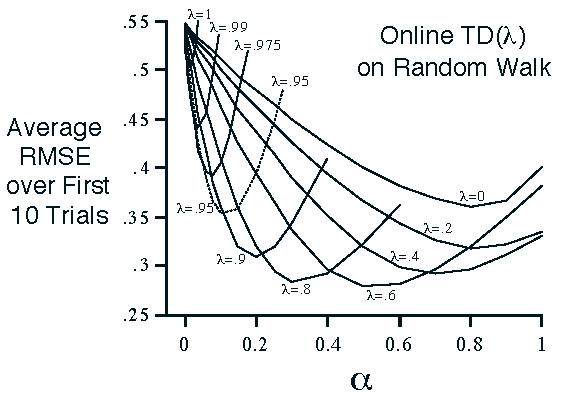
\includegraphics[width=0.7\textwidth]{Figures/TDlambda-tabular}
\ec
\uncover<+->{
Problem: 19-state random walk on a chain. Reward of $1$ at the left end. Both ends are absorbing. The goal is to predict the values of states.}
\note{
\bin
\item Learning rate is constant
\item Results for various $\lambda$ are shown.
\item \alert{Q1}: What can we conclude from the figure? (Intermediate values of $\lambda$ are better)
\item \alert{Q2}: Why does it hold that for smaller $\lambda$ the best $\alpha$ is larger?
\ei
}
}

\section{Function approximation}

\animframen{Too many states! What to do?}
{
\bi
\item The state space is too large
\bi
\item Cannot store all the values
\item Cannot visit all the states!
\ei
\item What to do???
\item Idea: Use compressed representations!
\item Examples
\bi
\item Discretization
\item Linear function approximation
\item Nearest neighbor methods
\item Kernel methods
\item Decision trees
\item $\vdots$
\ei
\item How to use them?
\ei
\note{
\bin
\item Mention ``Curse of dimensionality'' and its two meanings:
\bin
\item Computational (storage!) issues (FAPP overcomes)
\item Statistical issues (you need luck)
\ei
\item Draw the equations on the slide..
\item Illustrate with some graphics
\item For the future: animate linear function approximation 
\item[] (a point moves in 2D, the shape of the corresponding function is continuously updated)
\ei
}
}

\section{Methods}
\renewcommand{\t}{\theta}
\subsection{Stochastic gradient descent}

\animframejsqn{Regression \small with stochastic gradient descent}
{
\vspace*{-0.1in}
\bi
\item Assume $(\St_1,\Reward_1),(\St_2,\Reward_2),\ldots$ are i.i.d., $\exists V(\st) = \EE{ \Reward_t|\St_t=\st }$.
\item Goal: 
\bi 
\item Estimate $V$! 
\item With a function of the form $V_\theta(\st) = \theta^\top \phi(\st)$
\ei
\item This is called \alert{regression} in statistics/machine learning
\item \alert{More precise goal}: Minimize the expected squared prediction error:
\[
J(\t) = \tfrac12 \, \EE{ (\Reward_t - V_\t(\St_t))^2 }.
\]
\item Stochastic gradient descent:
\beqan
\t_{t+1} 
 &=& \t_t - \alpha_t  \tfrac12 \, \nabla_\t (\Reward_t - V_{\t_t}(\St_t))^2 \\
 &=& \t_t + \alpha_t (\Reward_t - V_{\t_t}(\St_t))\, \nabla_t  V_{\t_t}(\St_t) \\
 &=& \t_t + \alpha_t (\Reward_t - V_{\t_t}(\St_t))\, \phi(\St_t).
\eeqan
\item ``Robbins-Monro'' conditions:
$
\sum_{t=0}^\infty \alpha_t = \infty, \quad \sum_{t=0}^\infty \alpha_t^2 <\infty.
$
\ei
\note{
\tiny
\bin
	\item The main idea is that no precise information is needed to make a small step into the good direction in the weight space; on the average the direction is ok, errors are going to cancel out throughout the iterations
	\item \alert{Question}: What would be an alternative? 
	\bin
	\tiny
	\item Answer: Batching, i.e.,  find the minimizer of the empirical error based on the collected samples)
	\item OK if you have a small amount of data (data is expensive) and $\phi$ is low dimensional..
	\ei
	\item The second form with $\nabla_t  V_{\t_t}(\St_t)$ can be used e.g. with neural networks. Local minima then might be a problem;
	\item The main issue with stochastic gradient methods is when ``covariance matrix'' $\EE{\phi(\St_t)\phi(\St_t)^\top}$ is badly conditioned then it will zig-zag a lot on the error surface. The ``features'' do matter.
	\item Lot's of work recently in machine learning to speed up the process, e.g., mirror descent, matching losses, tuning the learning rate, higher order methods, etc.
	\item Under the RM conditions convergence (with linear function approximation) of the error(!) happens with probability one.
	\item If there is a unique solution, you converge to that.
	\item The error (squared!) converges at the rate $\dim(\phi)/t$. Cannot really improve. Tail bounds also exist. The parameter converges at the rate $1/\sqrt{t}$.
	\item 	
	\item If $\alpha_t \equiv {\rm const}$ small, then we have convergence in distribution to a random variables whose variance is proportional to $\alpha_t = \alpha_1$.
\ei
}
}

\animframen{Limit theory}
{
\bi
\item Stochastic gradient descent:
\beqan
\t_{t+1} - \t_t  &=& \alpha_t \, (\Reward_t - V_{\t_t}(\St_t))\, \phi(\St_t).
\eeqan
\item ``Robbins-Monro'' conditions:
$
\sum_{t=0}^\infty \alpha_t = \infty, \quad \sum_{t=0}^\infty \alpha_t^2 <\infty.
$
\item If converges, it must converge to $\t^*$ satisfying
\[
\EE{ (\Reward_t - V_{\t}(\St_t))\, \phi(\St_t) } = 0.
\]
\item Explicit form:
\[
\t^* = \EE{ \phi_t \phi_t\ttop }^{-1} \EE{ \phi_t \Reward_t },
\]
where $\phi_t = \phi(\St_t)$.
\item Indeed a minimizer of $J$.
\item ``LMS rule'', ``Widrow-Hoff'' rule, ``delta-rule'', ``ADALINE''
\ei
\emptynote
}

\subsection{TD($\lambda$) with linear function approximation}


\animframen{Learning from guesses: TD learning \small with function approximation}
{
\bi
\item Replace reward with return!
\item Idealistic Monte-Carlo based update:
\beqan
\t_{t+1} = \t_t + \alpha_t\, ( \Ret_t - V_{\t_t}(\St_t) ) \, \nabla_\t V_{\t_t}(\St_t)
\eeqan
where $\Ret_t$ is the return from state $\St_t$.
\item However, $\Ret_t$ is not available!
\item \alert{Idea}: Replace it with an estimate:
\beqan
\Ret_t  &\approx& \Reward_{t+1} + \gamma V_{\t_t}(\St_{t+1}).
\eeqan
\item Update:
\[
\t_{t+1} = \t_t + \alpha_t \,
	\overbrace{\left\{ \Reward_{t+1} + \gamma V_{\t_t}(\St_{t+1}) - V_{\t_t}(\St_t) \right\}}^{\alert{\delta_{t+1}(V_{\t_t})}}
	\, \nabla_\t V_{\t_t}(\St_t)
\]
\ei
\note{
\bin
\item We use the same bootstrap idea as before
\item Hence, this is \alert{not} a gradient algorithm
\item Theory says that 
\bin
\item It converges when used \alert{on-policy} (matching sampling distribution to the next-state distribution)
\item It might not converge when used \alert{off-policy}, see next slide
\ei
\item When $V_\theta$ is linear, $\nabla_{\t} V_{\t_t}(\St_t) = \phi(\St_t)$.
\item We get back the previous ``tabular'' algorithm when the state space is finite and $\phi(\st) = (\ldots,\one{\st=\st_k},\ldots)^\top$.
\item Where does it converge to when it converges? (We will see this later)
\item How about alternatives? (Bellman error methods) Not here, not now
\ei
}
}


\begin{frame}
\frametitle{TD($\lambda$) with linear function approximation}

        \begin{algorithmic}[1]
        \Statex \mbox{} \hspace*{-2em} {\bf function} \Call{TDLambdaLinFApp}{$\St,\Reward,\Nextstate,\theta,z$} 
	\Statex \mbox{} \hspace*{-2em} \textbf{Input:} $\St$ is the last state, $\Nextstate$ is the next state, $\Reward$ is the immediate reward associated with this transition, $\theta\in \real^d$  is the parameter vector of the linear function approximation, $z\in \real^d$ is the vector of eligibility traces
	\State $\delta  \gets \Reward+\gamma \,\cdot\, \theta\ttop \phi[\Nextstate] - \theta\ttop \phi[\St]$
	\label{algline:TD:td}
	\State $z \gets \phi[\St] + \gamma \,\cdot\,\lambda\,\cdot\, z$
	\State $\theta \gets \theta + \alpha \,\cdot\,\delta\,\cdot\, z$
	\State \Return $(\theta,z)$
	\end{algorithmic}
\note{
\bin
\item Complexity is linear in the number of features
\item[] This is important when we want to use a lot of features
\item There exists variants for action-value functions;
\item[] \alert{Question:} How would you do that?
\item How would you use this in learning to control (for the inpatients)
\ei
}
\end{frame}

\animframen{Issues with off-policy learning}
{
\bcol
\col
\bc
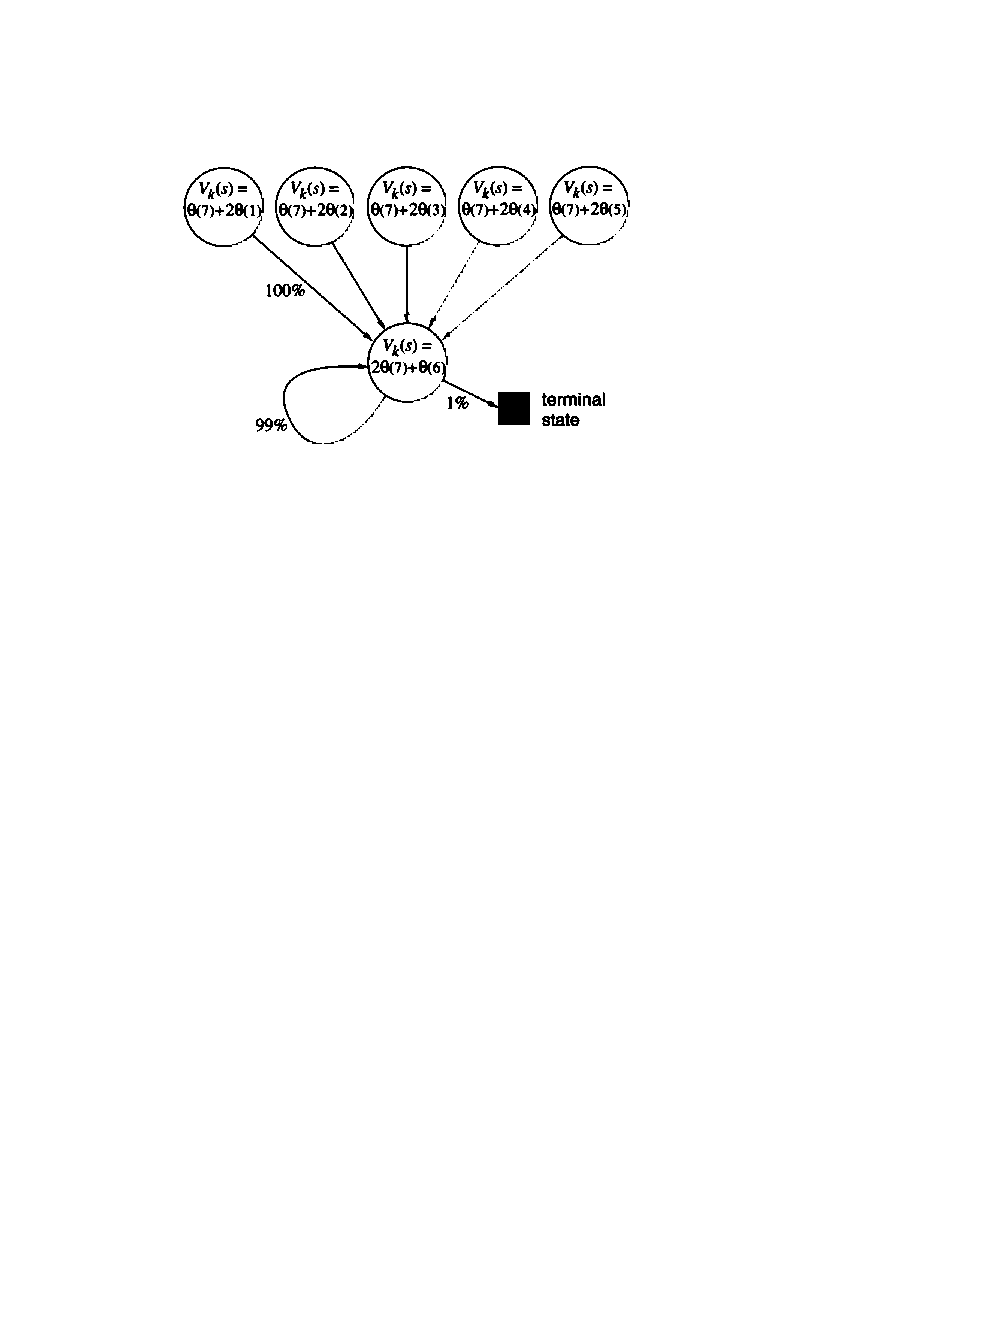
\includegraphics[width=\textwidth]{Figures/Baird-MDP}

$5$-star example
\ec
\col
\bc
\invisible<1>{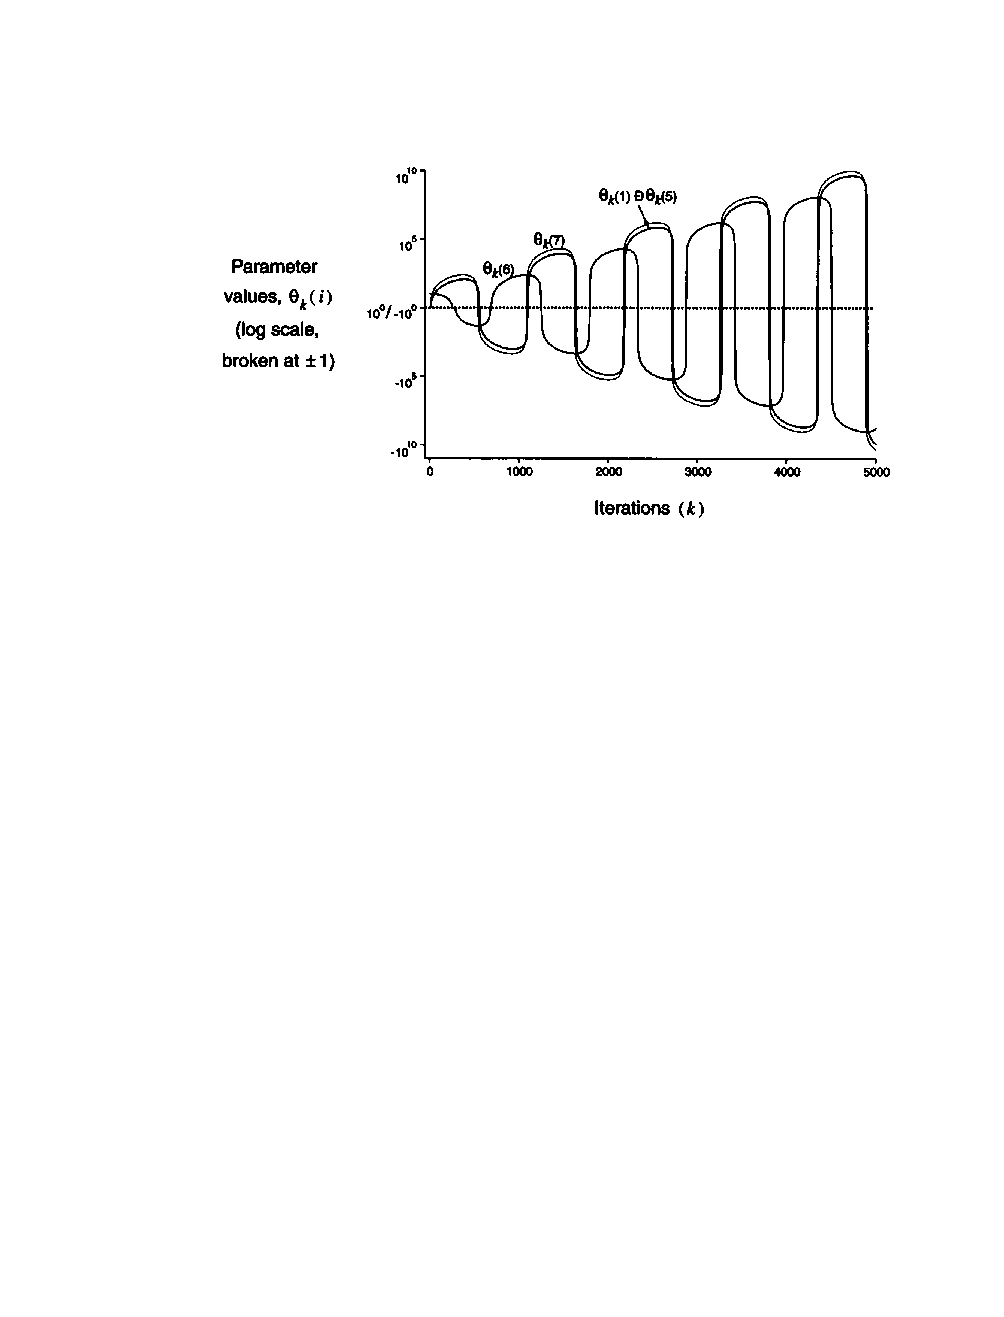
\includegraphics[width=\textwidth]{Figures/Baird-Values}}

\uncover<2->{
Behavior of TD(0) with expected backups on the $5$-star example}
\ec
\ecol
\note{
\bin
\item This is known as ``Baird's counterexample''
\item Tsitsiklis and Van Roy have a two-state counterexample:
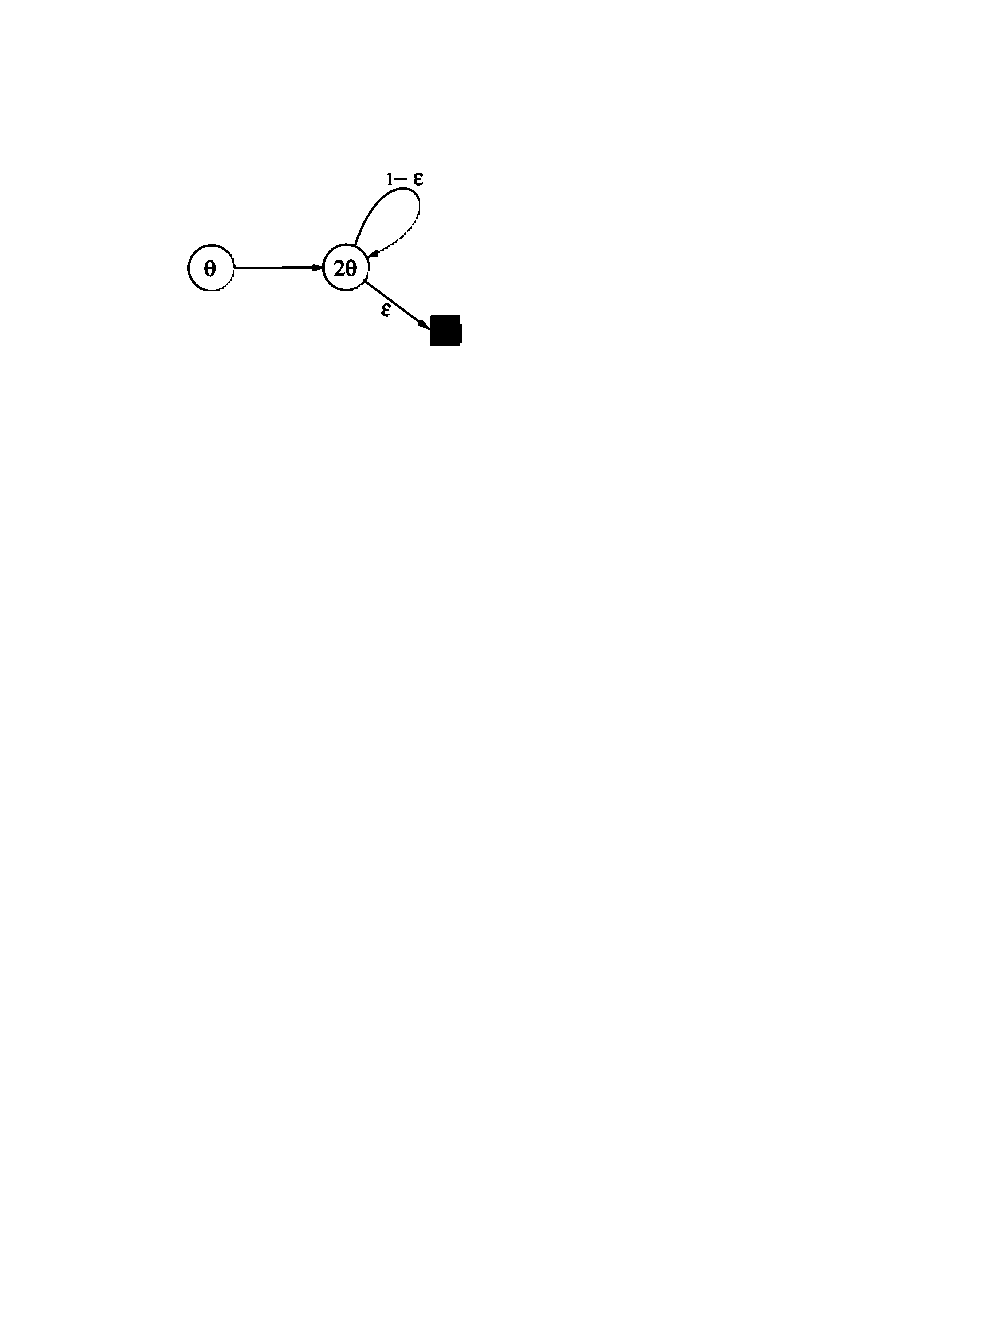
\includegraphics[width=0.3\textwidth]{Figures/Tsitsiklis-VanRoy-MDP}
\item Then fitted value iteration can be easily seen to diverge
\item The example also works for TD
\item The convergence of TD is actually governed by the ODE
\[
\dot\t = -A\t + b,
\]
where $A = \EE{ (\phi(\St_t)- \gamma \phi(\St_{t+1}')  ) \phi(\St_t)\ttop }$,
$b = \EE{ \Reward_{t+1} \phi(\St_t) }$, assuming stationary data.
\bin
\item If $-A$ is negative stable, the ODE converges and so does TD(0).
\item In the other case, both will diverge
\item Note that $A$ is non-symmetric!
\ei
% TODO add citations
\ei
}
}

\subsection{Gradient temporal difference learning}

\animframen{Defining the objective function}
{
\bi
\item Let 
$\delta_{t+1}(\theta) =
 \Reward_{t+1} + \gamma V_\theta(\Nextstate_{t+1}) - V_\theta(\St_t)$ be the TD-error at time $t$, $\phi_t = \phi(\St_t)$.
\item TD(0) update:
\[
\t_{t+1} - \t_t = \alpha_t \, \delta_{t+1}(\t_t) \phi_t.
\]
\item When TD(0) converges, it converges to a unique vector $\theta^*$ that satisfies 
\beq
\EE{\delta_{t+1}(\theta^*) \phi_t} =0. \tag{TDEQ}
\eeq
\item \alert{Goal}: Come up with an objective function such that its optima satisfy~(TDEQ).
\item Solution:
\[
J(\t) =  \EE{\delta_{t+1}(\t) \phi_t }\ttop \EE{\phi_t \phi_t\ttop }^{-1} \EE{ \delta_{t+1}(\t) \phi_t }.
\]
\ei
}

\animframen{Deriving the algorithm}
{
\[
J(\t) =  \EE{\delta_{t+1}(\t) \phi_t }\ttop \EE{\phi_t \phi_t\ttop }^{-1} \EE{ \delta_{t+1}(\t) \phi_t }.
\]
\bi
\item Take the gradient!
\[
\nabla_\theta J(\theta) = - 2 \EE{ (\phi_t - \gamma \phi_{t+1}') \phi_t\ttop } w(\theta),
\]
where 
\[
w(\theta) = \EE{\phi_t \phi_t\ttop }^{-1} \EE{ \delta_{t+1}(\theta) \phi_t }.
\]
\item \alert{Idea}: introduce two sets of weights!
\beqan
\uncover<.->{\theta_{t+1} }
	&\uncover<.->{=}&
	\uncover<.->{\theta_t + \alpha_t \, \cdot\, (\phi_t - \gamma \,\cdot\, \phi_{t+1}') \,\cdot\, \phi_t\ttop w_t} \\
\uncover<+->{w_{t+1}}
    &\uncover<.->{=}& 
    \uncover<.->{w_t + \beta_t \,\cdot\, ( \delta_{t+1}(\t_t) -  \phi_t\ttop w_t )\,\cdot\, \phi_t.}
\eeqan
\ei
\note{
\bin
\item Update rule of $w_t$: Just stochastic gradient rule (assuming $\t_t$ is kept fixed).
\item We have two step-size sequences! Tuning maybe more difficult.
\item Good thing: The algorithm converges (to the desired solution) 
		as long as the step-size sequences satisfy the RM conditions.
\item[] This is actually lucky..
\ei
}
}

\begin{frame}
\frametitle{GTD2 with linear function approximation}

        \begin{algorithmic}[1]
        \Statex \mbox{} \hspace*{-2em} {\bf function} \Call{GTD2}{$\St,\Reward,\Nextstate,\theta,w$} 
	\Statex \mbox{} \hspace*{-2em} \textbf{Input:} $\St$ is the last state, $\Nextstate$ is the next state, $\Reward$ is the immediate reward associated with this transition, $\theta\in \real^d$  is the parameter vector of the linear function approximation, $w\in \real^d$ is the auxiliary weight
	\State $f \gets \phi[\St]$
	\State $f' \gets \phi[\Nextstate]$
	\State $\delta  \gets \Reward+\gamma \,\cdot\, \theta\ttop f' - \theta\ttop f$
	\State $a \gets f\ttop w$
	\State $\theta \gets \theta + \alpha \, \cdot\, (f - \gamma \,\cdot\, f') \,\cdot\, a$ \label{algline:GTD2:uptheta}
	\State $w \gets w + \beta \,\cdot\, ( \delta - a )\,\cdot\, f$
	\State \Return $(\theta,w)$
	\end{algorithmic}

\note{
\bin
\item Complexity is twice the complexity of TD.
\item Still linear
\item There exists variants for action-value functions
\item[] \alert{Question:} How would you do that?
\item The underlying ODE is
\[
\frac{d}{dt} \begin{pmatrix} d \\ \t \end{pmatrix} =
G \begin{pmatrix} d \\ \t \end{pmatrix}
+ \begin{pmatrix} b \\ 0 \end{pmatrix},
\]
where $d=w/\sqrt{\eta}$,
\[
G = \begin{pmatrix} -\sqrt{\eta} C & - A \\ A\ttop & 0 \end{pmatrix},
\]
and  $\beta_t = \eta \alpha_t$.
\ei
}
\end{frame}

\animframen{Experimental results}
{
\bcol
\col
\bc
\uncover<+->{
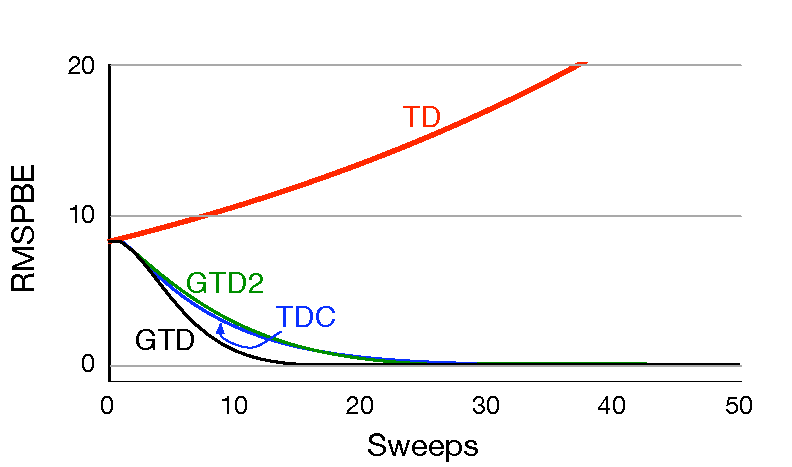
\includegraphics[width=0.9\textwidth]{Figures/GTD-Baird}

Behavior on $7$-star example}
\ec
\col
\bc
\invisible<1>{
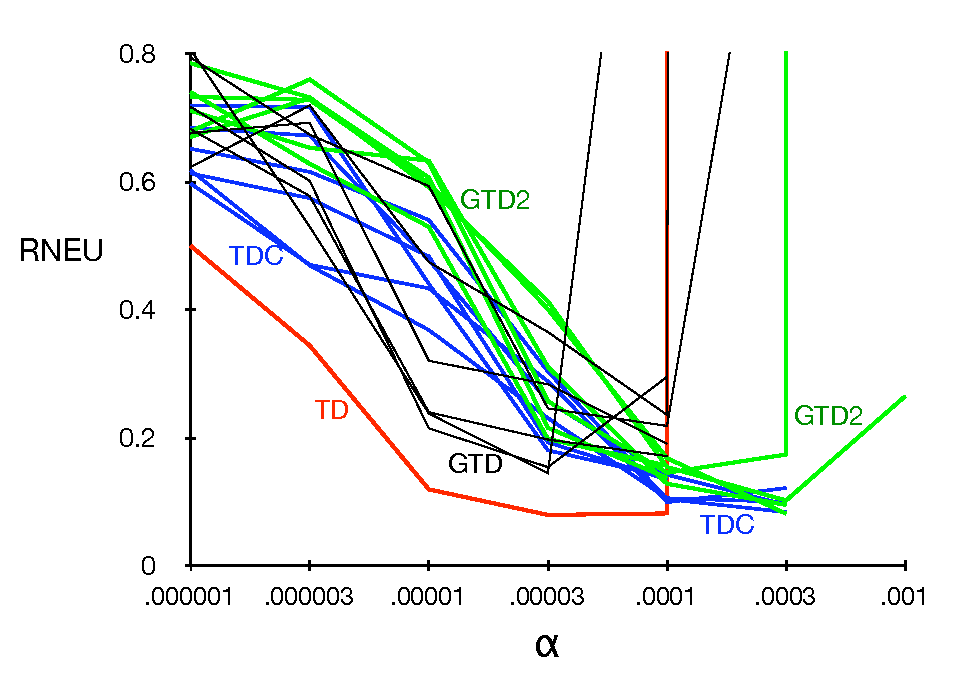
\includegraphics[width=0.9\textwidth]{Figures/GTD-Goresults}

Behavior on Computer Go}
\ec
\ecol

\note{
\vspace*{-0.2in}
\tiny
\bin
\item Sanity check no. 1; off-policy case
\bin \tiny
\item 7-state version of the �star� counterexample from Baird (1995)
\item Updating: synchronously
in dynamic-programming-like sweeps through the
state space. 
\item For TD, $\alpha = 0.1$. 
\item For the gradient algorithms,
$\alpha = 0.05$ and $\eta = 10$. 
\item The initial parameter value was '$\t_0 =(1, 1, 1, 1, 1, 1, 10, 1)\ttop$, and $\gamma = 0.99.$
\ei
\item Sanity check no. 2; on-policy case:
\bin \tiny
\item Goal is to be competitive with TD, which is still a pretty good algorithm
\item $9\times 9$ Computer Go, RLGO, purely linear value functions
\item $969,894$ binary features corresponding to all possible shapes in every $3\times 3$, $2\times 2$, and $1\times 1$ region of the board
\item Using weight sharing
to take advantage of location-independent and location dependent
symmetries, the million features are reduced to
a parameter vector of $n = 63,303$ components.
\item Policy to evaluate: Random play, self-play
\item Winning gives a reward of $1$
\item NEU($\theta$) $\equiv \|\EE{ \delta(\theta) \phi }\|$, estimated over $1000$ test games
\item[] NEU = ``Norm of Expected Update''
\item Experiment repeated $40$ times, averages of NEU are shown
\ei
\ei
}
}

\animframen{Bibliographic notes and subsequent developments}
{
\bi
\item GTD -- the original idea \citep{SuSzeMa08}
\item GTD2, a two-timescale version (\alert{TDC}) \citep{Suetal:ICML09}.
\item[] Just replace the update in line~\ref{algline:GTD2:uptheta} by
\[
 \qquad \theta \gets \theta + \alpha \, \cdot\, (\delta\,\cdot\, f  - \gamma \,\cdot\, a \,\cdot\,f').
\]
\item Extension to nonlinear function approximation \citep{Maetal:09}
\item[] Addresses the issue that TD is unstable when used with nonlinear function approximation
\item Extension to eligibility traces, action-values \citep{MaSut10}
\item Extension to control (next part!)
\ei
\note{
% TODO: Add citations
}
}

\subsection{LSTD and friends}


\animframen{The problem}
{
\bi
\item The methods are ``gradient''-like, or ``first-order methods''
\item Make small steps in the weight space
\item They are sensitive to:
\bi
\item choice of the step-size
\item initial values of weights
\item eigenvalue spread of the underlying matrix determining the dynamics
\ei
\item Solution proposals:
\bi
\item Use of adaptive step-sizes \citep{Sutton92:GainAdaptation,GePo06}
\item Normalizing the updates \citep{bradtke94}
\item Reusing previous samples \citep{Lin92}
\ei
\item Each of them have their own weaknesses
\ei
\note{
\bin
\item Weaknesses:
\bin
\item Adaptive step-size: No guarantees, still sensitive, cannot correct for huge eigenvalue spread
\item Normalizing the updates: same
\item Reusing previous samples: Two much computation, still requires step-sizes, $\ldots$
\ei
\ei
}
}

\animframejsqn{The LSTD algorithm}
{
\bi
\item In the limit, if TD($0$) converges it  finds the solution to
$\alert{(*)} \quad \EE{ \,\phi_t\, \delta_{t+1}(\theta)\, } = 0.$
\item Assume the sample so far is
\[\Sample_n = 
((\St_0,\Reward_{1},\Nextstate_{1}),
 (\St_1,\Reward_{2},\Nextstate_{2}),
\ldots,
(\St_{n-1},\Reward_{n},\Nextstate_{n})),
%((\St_t,\Reward_{t+1},\Nextstate_{t+1});t\in \{0,\ldots,n-1\})
\]
\item \alert{Idea}: Approximate~(*) by $\qquad$
$\alert{(**)} \quad
\frac1n \sum_{t=0}^{n-1} \phi_t\, \delta_{t+1}(\theta)  = 0.
$
\bi
\item \tiny Stochastic programming:  {\em sample average approximation} \citep{Shapiro03}
\item \tiny Statistics: $Z$-estimation \citep[e.g.,][Section~2.2.5]{Kosorok08}
\ei
\item Note: (**) is equivalent to
\[
-\hA_n \t + \hb_n = 0,
\]
where
	$\hb_n = \frac1n \sum_{t=0}^{n-1}R_{t+1} \phi_t $ and 
	$\hA_n = \frac1n \sum_{t=0}^{n-1} \phi_t(\phi_t-\gamma \phi_{t+1}')\ttop$.
\item Solution:
$\theta_n = \hA_n^{-1} \hb_n$, provided the inverse exists.
\item \alert{Least-squares temporal difference} learning or LSTD \citep{BraBa96}.
\ei
\note{
\bi
\item The original equation may not have a solution!
\item LSTD minimizes the empirical approximation to the projected squared Bellman error, $\norm{\Pi_{\FF,\dstat} (T V - V)}_{\dstat}^2$,
over the linear space $\FF$
\citep{anszemu:mlj07}.
\item This criterion is always well defined (GTD2 and TDC use it too!)
\item The Sherman-Morrison formula (matrix inversion lemma) allows one to update the weight
vector incrementally
\item The resulting algorithm is the counterpart of ``Recursive least-squares'' in adaptive filtering (RLS~LMS, LSTD~TD)
\item The LSTD($\lambda$) solution is derived from the TD($\lambda$) update:
\[
\frac1n \sum_{t=0}^{n-1} \delta_{t+1}(\theta) \elg_{t+1} = 0,
\elg_{t+1} = \sum_{s=0}^t (\gamma \lambda)^{t-s} \phi_s.
\]
\item There is an incremental (recursive) form, too.
\ei
}
}

\begin{frame}
\frametitle{RLSTD($0$) with linear function approximation}

        \begin{algorithmic}[1]
        \Statex \mbox{} \hspace*{-2em} {\bf function} \Call{RLSTD}{$\St,\Reward,\Nextstate,C,\theta$} 
	\Statex \mbox{} \hspace*{-2em} \textbf{Input:} $\St$ is the last state, $\Nextstate$ is the next state, $\Reward$ is the immediate reward associated with this transition, $C\in \real^{d\times d}$, and $\theta\in \real^d$  is the parameter vector of the linear function approximation
	\State $f \gets \phi[\St]$
	\State $f' \gets \phi[\Nextstate]$
	\State $g \gets (f-\gamma f')\ttop C$ \Comment{$g$ is a $1\times d$ row vector}
	\State $a \gets  1+g f $
	\State $v \gets C f$
	\State $\delta  \gets \Reward+\gamma \,\cdot\, \theta\ttop f' - \theta\ttop f$
	\State $\theta \gets \theta + \delta\,/\, a\,\cdot\, v$
	\State $C \gets C - v \, g  \,\,/\, a$
	\State \Return $(C,\theta)$
	\end{algorithmic}
\note{
\bin
\item $\lambda$-LSPE due to Bertsekas and Ioffe (1996) mixes incremental updates and optimization updates. The optimization is done in a fitted-value iteration manner based on multi-step prediction of values:
\[
\hat{V}_{s,n}^{(\lambda)}(\theta) =
\theta\ttop \phi_s  + \sum_{q=s}^{n-1} (\gamma \lambda)^{q-s}\, \delta_{q+1}(\theta)
\]
\ei
}
\end{frame}

\subsection{Comparing least-squares and TD-like methods}
\animframesqn{Which one to love?}
{
\begin{block}{Assumptions}
\vspace*{-0.4in}
\bcol
\col
\bi
	\item Time for computation $T$ is fixed
\ei
\col
\bi
	\item Samples are cheap to obtain 
	%(e.g., an efficient simulator is available), i.e., sample size is not fixed
\ei
\ecol
\end{block}

\begin{block}{Some facts}
\bcol
\col
How many samples ($n$) can be processed?
	\bi
		\item Least-squares: $n \approx T/d^2$
		\item First-order methods: $n' \approx  T/d = n d$
	\ei
\col
 Precision after $t$ samples?
	\bi
		\item Least-squares: $C_{1} t^{-\frac12}$
		\item First-order: $C_{2} t^{-\frac12}$
		\item $C_2>C_1$
	\ei
\ecol
\end{block}
\begin{block}{Conclusion}
Ratio of precisions:
	\[
		\frac{\|\theta_{n'}'-\theta_*\|}{\|\theta_n-\theta_*\|} \,\approx\,\, \frac{C_2}{C_1}\,\, d^{-\frac12},
	\]
Hence:
{\em If $C_2/C_1 < d^{1/2}$ then the first-order method wins, 
				in the other case the least-squares method wins.}
\end{block}

\note{
\bin
	\item It is difficult to decide which method (least-squares or first-order) will work better {\em a priori}.
	\item Rule of thumb:
	\bin
		\item if $d$ is small, least-squares methods may win
		\item  if $d$ is large, first-order methods may win
	\ei
	\item This analysis is not specific to RL, but holds in supervised learning, too,
	\item Here $\theta_{n'}'$ is the parameter found by the first-order method
	\item[] $\theta_{n}$ is the parameter found by the least-squares method
% see \citealp{BoBo07})
%	\item iLSTD tries to merge the best of both worlds \citep{GeBoZiSu06}
\ei
}
}

\section{How to choose the function approximation method?}
\animframen{The choice of the function approximation method}
{
\begin{block}{Factors to consider}
\bi
\item Quality of the solution in the limit of infinitely many samples
\item Overfitting/underfitting
\item ``Eigenvalue spread'' (decorrelated features) when using first-order methods
\ei
\end{block}

\note{
\bin
\item Overfitting/underfitting: when you use lots of features, with few samples you can easily overfit
\item[] Good methods should prevent this
\item[] Incremental methods help a bit in this respect
\item[] ``Regularization''  can help the other methods
\item Eigenvalue spread: This is not much studied.. The real parts of the eigenvalues of $A$ should be clustered together to allow maximal rate of convergence
\ei
}
}
\animframen{Error bounds}
{
\begin{block}{} %{Limiting behavior I.}
Consider TD($\lambda$) estimating the value function $V$.
Let $V_{\theta^{(\lambda)}}$ be the limiting solution. Then
\[
\norm{V_{\theta^{(\lambda)}} - V }_\dstat \le 
%\frac{1-\gamma \lambda}{1-\gamma }
\frac{1}{\sqrt{1-\gamma_\lambda}}
\, 
\norm{\Pi_{\FF,\dstat} V - V }_\dstat.
\]
Here $\gamma_\lambda = \gamma(1-\lambda)/(1-\lambda\gamma)$ is the contraction modulus of 
$\Pi_{\FF,\dstat} T^{(\lambda)}$ \citep{TsiVR99,Ber07:DPbookVol2}.
\end{block}
\note{
Sharper bounds are available, e.g., due to Yu and Bertsekas  (2008).
}
}

\if0
\animframen{TD($\lambda$) solves a model}
{
\bi
\item \alert{Linear model}: 
State space $\ZZ = \real^d$; linear immediate rewards $\reward(z) =  \ip{b^{(\lambda)}}{z}$;
 linear, deterministic transitions $z \mapsto A^{(\lambda)} z$. 
 \item Bellman equation:
\[
V(z) = \ip{b^{(\lambda)}}{ z} +\gamma\, V( A^{(\lambda)} z ), \quad z\in \real^d.
\]
\item If there exists a solution, there exists a linear solution:
\beq\label{eq:linbellman}
\ip{\theta^{(\lambda)}}{z} =  
\ip{b^{(\lambda)}}{ z} +\gamma\, \ip{\theta^{(\lambda)}}{A^{(\lambda)} z}, 
\quad z\in \real^d.
\eeq
\item \alert{Claim}: If $\t^{(\lambda}$ is the limiting parameter vector found by TD($\lambda$) 
then it satisfies~\eqref{eq:linbellman} with an appropriate model.
\item Note: The case of $\lambda=0$ is treated in \citet{SuSzGeBo08} and \citet{PalITaPWLi08}.
\ei
\note{
\bin
\item So what??
\ei
}
}
\fi


\animframen{Error analysis II}
{
%\citet{PalITaPWLi08}
\bi
\item Define the \alert{Bellman error}
$\Delta^{(\lambda)}(\hV)=T^{(\lambda)} \hV - \hV$,
 $\hV:\States\ra\real$
under $T^{(\lambda)} = 
(1-\lambda) \sum_{m=0}^\infty \lambda^m \,T^{[m]}$, where $T^{[m]}$ is the \alert{$m$-step lookahead Bellman operator}.
\item Contraction argument:
 $\norm{V-\hV}_\infty \le \frac{1}{1-\gamma}\, \norm{\Delta^{(\lambda)}(\hV)}_\infty$.
\item What makes $\Delta^{(\lambda)}(\hV)$ small?
\item Error decomposition:
\[
\Delta^{(\lambda)}(V_{\theta^{(\lambda)}}) = 
(1-\lambda) \sum_{m\ge 0}\lambda^m  \Delta^{[r]}_m +
 \gamma \,
\left\{(1-\lambda) \sum_{m\ge 0}\lambda^m  \Delta_{m}^{[\phi]}\right\} \theta^{(\lambda)},
\]
where
\bi[<.->]
\item $\Delta^{[r]}_m=\overline{r}_m-\Pi_{\FF,\dstat} \overline{r}_m$
\item $ \Delta^{[\phi]}_m = P^{m+1}  \phi\ttop   - \Pi_{\FF,\dstat} P^{m+1}  \phi\ttop$
\item $\overline{\reward}_m(\st) = \EE{ \Reward_{m+1} \,|\,\St_0 = \st}$,
\item $P^{m+1} \phi\ttop (\st) = (P^{m+1} \phi_1(\st),\ldots,P^{m+1}\phi_d(\st))$,
\item $P^m \phi_i(\st) = \EE{ \phi_i(\St_{m}) \,|\, \St_0 = \st}$.
\ei
\ei

\note{
\bin
\item $m$-step lookahead Bellman operator:
\[
T^{[m]} \hV \,(\st) 
= \EE{  \sum_{t=0}^m \gamma^t \Reward_{t+1} + \gamma^{m+1} \,\hV(\St_{m+1}) \,\Big|\, \St_0 = \st }.
\]
\item Thus, we see that the Bellman error will be small 
if the $m$-step immediate rewards
and the $m$-step feature-expectations are well captured
by the features. 
\item As $\lambda$ gets closer to $1$, it becomes more important for the features to capture the structure of the value function, and as $\lambda$ gets closer to $0$, it becomes more important to capture the structure of the immediate rewards and the immediate feature-expectations.
\item This gives us some hint on how to choose the features and $\lambda$!
\ei
}

}


\section{Bibliography}
\begin{frame}
  \frametitle{For Further Reading}
  \begin{multicols}{2}
  \scriptsize\tiny
\def\newblock{\hskip .11em plus .33em minus .07em}
\bibliography{allbib,shortconfs}
  \end{multicols}
\emptynote
\end{frame}

\end{document}
